\documentclass[11pt,a4paper]{article}
\usepackage[T1]{fontenc}
\usepackage[utf8]{inputenc}
\usepackage{lmodern}
\usepackage[margin=27mm]{geometry}
\usepackage{amsmath,amssymb,amsthm,mathtools}
\usepackage{microtype,booktabs,array,longtable,enumitem}
\usepackage{tikz}
\usetikzlibrary{arrows.meta,positioning,calc}
\usepackage[unicode,hidelinks]{hyperref}
\hypersetup{pdftitle={Prescribed large-volume charges on threefolds with trivial canonical bundle},pdfauthor={OpenAI}}
\pdfinfoomitdate=1
\pdftrailerid{}
\pdfsuppressptexinfo=15
\input{glyphtounicode}
\pdfgentounicode=1
\pdfglyphtounicode{parenleftbig}{0028}
\pdfglyphtounicode{parenrightbig}{0029}
\pdfglyphtounicode{bracketleftbig}{005B}
\pdfglyphtounicode{bracketrightbig}{005D}
\pdfglyphtounicode{parenleftBig}{0028}
\pdfglyphtounicode{parenrightBig}{0029}
\pdfglyphtounicode{parenleftbigg}{0028}
\pdfglyphtounicode{parenrightbigg}{0029}
\pdfglyphtounicode{angbracketleftbigg}{27E8}
\pdfglyphtounicode{angbracketrightbigg}{27E9}
\pdfglyphtounicode{parenleftBigg}{0028}
\pdfglyphtounicode{parenrightBigg}{0029}
\pdfglyphtounicode{braceleftBigg}{007B}
\pdfglyphtounicode{bracerightBigg}{007D}
\pdfglyphtounicode{angbracketleftBigg}{27E8}
\pdfglyphtounicode{angbracketrightBigg}{27E9}
\pdfglyphtounicode{summationtext}{2211}
\pdfglyphtounicode{producttext}{220F}
\pdfglyphtounicode{integraltext}{222B}
\pdfglyphtounicode{summationdisplay}{2211}
\pdfglyphtounicode{productdisplay}{220F}
\pdfglyphtounicode{integraldisplay}{222B}
\pdfglyphtounicode{hatwide}{0302}
\pdfglyphtounicode{tildewide}{0303}
\pdfglyphtounicode{radicalbig}{221A}
\pdfglyphtounicode{radicalBig}{221A}
\pdfglyphtounicode{vextenddouble}{20E6}
\setlength{\emergencystretch}{2em}
\numberwithin{equation}{section}
\newtheorem{theorem}{Theorem}[section]
\newtheorem{proposition}[theorem]{Proposition}
\newtheorem{lemma}[theorem]{Lemma}
\newtheorem{corollary}[theorem]{Corollary}
\theoremstyle{definition}
\newtheorem{definition}[theorem]{Definition}
\theoremstyle{remark}
\newtheorem{remark}[theorem]{Remark}
\DeclareMathOperator{\ch}{ch}
\DeclareMathOperator{\td}{td}
\DeclareMathOperator{\rk}{rk}
\DeclareMathOperator{\Hom}{Hom}
\DeclareMathOperator{\Ext}{Ext}
\DeclareMathOperator{\Coh}{Coh}
\DeclareMathOperator{\Stab}{Stab}
\DeclareMathOperator{\Spec}{Spec}
\DeclareMathOperator{\im}{im}
\DeclareMathOperator{\supp}{Supp}
\newcommand{\OO}{\mathcal O}
\newcommand{\CC}{\mathbb C}
\newcommand{\RR}{\mathbb R}
\newcommand{\QQ}{\mathbb Q}
\newcommand{\ZZ}{\mathbb Z}
\newcommand{\HH}{\mathbb H}
\newcommand{\Db}{D^{\mathrm b}}
\newcommand{\Knum}{K_{\mathrm{num}}}
\title{Prescribed large-volume charges on threefolds with trivial canonical bundle}
\author{OpenAI}
\date{September 24, 2026}
\begin{document}
\maketitle
\begin{abstract}
Let $X$ be a smooth projective complex threefold with trivial canonical
bundle. We construct numerical Bridgeland stability conditions with the exact
ordinary and square-root-Todd central charges at every sufficiently large
volume. One volume threshold works on an open set of real twists and ample
directions. The resulting stability conditions have the support property on
the full numerical Grothendieck group and stable point sheaves. Separately, on
every smooth projective complex threefold we prove a strong tilt inequality
above a volume threshold uniform in the object and twist along a fixed
polarization.
\end{abstract}
\tableofcontents
\section{Introduction}\label{sec:introduction}

A central charge assigns a complex number to each object of a derived
category. A stability condition organizes the objects by its argument and
requires every object to have a finite filtration by semistable factors.
Bridgeland introduced this structure and its deformation theory
\cite{Bridgeland2007}. On a projective threefold, the expected large-volume
charges are exponential expressions in the Chern character. The
prescribed-charge problem asks whether these particular expressions admit
a compatible heart, finite semistable filtrations, and a support bound
controlling the numerical classes of all semistable objects.

We construct stability conditions with the exact ordinary and
square-root-Todd large-volume charges on every smooth projective complex
threefold with trivial canonical bundle. One volume threshold works on an
open set of real twists and real ample directions. The support property
holds on the full numerical Grothendieck group, and the ordinary charge
has the standard double-tilt heart. An independent argument proves strong
tilt inequalities on every smooth projective complex threefold: a fixed
rational correction works at every volume, and the correction vanishes
beyond a threshold independent of the object and of the twist along a
fixed polarization.

All varieties are over $\CC$, and all Chern characters and intersection
products are numerical. Write $N^1(X)_{\RR}$ for the space of numerical
real divisor classes, $\operatorname{Amp}(X)$ for its ample cone, and
$N_1(X)_{\QQ}$ for the space of numerical rational curve classes.
A threefold is smooth, connected and projective.
The assertions for a disjoint union follow by applying the results to
its finitely many connected components and taking the largest constants.
Write $\Db(X)=\Db\Coh(X)$ and
$\ch^B(E)=e^{-B}\ch(E)$ for a real numerical divisor class $B$.

\subsection{Prescribed charges and the full numerical group}

The Euler pairing is
$\chi(E,F)=\sum_j(-1)^j\dim\Ext^j(E,F)$, and we use
\[
 \Knum(X)=K_0(X)/\{v:\chi(v,w)=0\text{ for every }w\in K_0(X)\}.
\]
A numerical stability condition consists of a charge homomorphism
$Z:\Knum(X)\to\CC$ and a locally finite slicing $\mathcal P$ of
$\Db(X)$. A slicing gives the semistable objects of each real phase,
with $Z(E)=m(E)e^{i\pi\phi}$, $m(E)>0$, on $\mathcal P(\phi)$,
the shift and Hom-vanishing rules, and finite Harder--Narasimhan
filtrations. Local finiteness requires the categories of sufficiently
short phase intervals to have finite length. We require the support
property of Kontsevich--Soibelman
\cite[Sections~1.2 and~2.1]{KontsevichSoibelman2008} on the full real space
$\Knum(X)_{\RR}$: for a norm there is $C>0$ such that
$\|[E]\|\leq C|Z(E)|$ for every semistable $E$.
Its heart is $\mathcal P(0,1]$. We call a stability condition geometric
if all point sheaves $\OO_x$ are stable of phase $1$.

We specify the tilt conventions needed to state the heart in our theorem.
For a real ample class $H$, a real divisor class $B$, and a coherent sheaf
of positive rank put
\[
 \mu_{H,B}(F)=\frac{H^2\ch_1^B(F)}{H^3\ch_0(F)},
\]
and give a nonzero torsion sheaf slope $+\infty$.
The slope Harder--Narasimhan filtration has semistable factors of strictly
decreasing slopes; write $\mu^+$ and $\mu^-$ for its largest and smallest
slopes. The slope torsion pair and its tilt are
\[
 \mathcal T_{H,B}=\{F:\mu^-_{H,B}(F)>0\},\qquad
 \mathcal F_{H,B}=\{F:\mu^+_{H,B}(F)\leq0\},\qquad
 \mathcal B_{H,B}=\langle\mathcal F_{H,B}[1],\mathcal T_{H,B}\rangle,
\]
with the zero sheaf in both subcategories. Here a heart is the abelian
category specified by a bounded $t$-structure, $[1]$ is the cohomological
shift, and brackets denote extension closure. Thus an object of
$\mathcal B_{H,B}$ has ordinary cohomology only in degrees $-1,0$, in the
indicated two subcategories.

For real $B$, real ample $H$ and $t>0$, the ordinary physical charge is
\begin{equation}\label{eq:intro-physical}
 Z_{B,tH}(E)=
 -\ch_3^B(E)+\frac{t^2}{2}H^2\ch_1^B(E)
 +i\left(tH\ch_2^B(E)-\frac{t^3}{6}H^3\ch_0(E)\right).
\end{equation}
The first tilt is unchanged if the polarization $H$ is replaced by
$tH$. On this first tilt, use the second slope
\[
 \nu_{B,tH}(E)=
 \frac{tH\ch_2^B(E)-t^3H^3\ch_0(E)/6}{t^2H^2\ch_1^B(E)}.
\]
Its denominator-zero value is $+\infty$. An object is semistable for
this slope if every nonzero proper subobject in $\mathcal B_{H,B}$ has
slope at most that of the quotient; stability uses a strict inequality.
The Harder--Narasimhan property holds for these real ample parameters
\cite[Section~2]{BMS2016}. Let $\mathcal T'_{B,tH}$
have strictly positive smallest Harder--Narasimhan slope, and
$\mathcal F'_{B,tH}$ have nonpositive largest slope. The standard
double-tilt heart is
\[
 \mathcal A_{B,tH}=
 \langle\mathcal F'_{B,tH}[1],\mathcal T'_{B,tH}\rangle.
\]
These definitions use the same strict-positive/nonpositive boundary
at both tilts.

\begin{theorem}[Exact large-volume charges on a real sector]
\label{thm:geometric-sector}
Let $X$ be a smooth projective complex threefold with
$K_X\simeq\OO_X$. For any $B_*\in N^1(X)_{\RR}$ and
$H_*\in\operatorname{Amp}(X)$ there are open neighborhoods $V$ of
$B_*$ and $W$ of $H_*$ and one $T>0$ such that, for all
$B\in V$, $H\in W$ and $t\geq T$, the following hold.
\begin{enumerate}[label=\textup{(\roman*)}]
\item $(Z_{B,tH},\mathcal A_{B,tH})$ is a geometric numerical
stability condition with support on $\Knum(X)_{\RR}$.
\item There is a geometric numerical stability condition, with support
on the same full numerical space, whose charge is exactly
\[
 Z^{\mathrm{LV}}_{B,tH}(E)
 =-\int_Xe^{-B-itH}\ch(E)\sqrt{\td(X)},
 \qquad \sqrt{\td(X)}=1+\frac{c_2(X)}{24}.
\]
Its heart is the one constructed in Section~\ref{sec:ambient}.
\end{enumerate}
\end{theorem}

Only triviality of $K_X$ is assumed; the additional vanishings
$H^1(X,\OO_X)=H^2(X,\OO_X)=0$ in the strict Calabi--Yau convention
are unnecessary. The quantifiers give one threshold for both charges
throughout the same real sector. The two hearts are specified separately:
the ordinary charge uses the double tilt defined above, while the
Todd-corrected charge uses the heart constructed in
Section~\ref{sec:ambient}.

The ordinary and square-root-Todd charges have large-volume antecedents in
Bayer's polynomial stability conditions
\cite[Theorem~3.2.2 and Section~4]{BayerPolynomial2009}. Polynomial stability
orders phases asymptotically as the volume tends to infinity. Our theorem
constructs a numerical Bridgeland stability condition at each finite
volume in the stated sector. The passage to finite volume must also
control the charge kernel: on a threefold of Picard rank greater than
one, the full numerical group contains classes invisible to the four
intersection degrees along a single polarization.

\subsection{Independent uniform tilt inequalities}

The numerical problem concerns the third Chern character, which is absent
from the classical Bogomolov--Gieseker inequality. Bayer--Macr\`i--Toda
introduced the double-tilt construction and proposed a third-character
inequality that would make it a source of stability
conditions~\cite{BMT2014}. Bayer--Macr\`i--Stellari established that
inequality for abelian threefolds and Calabi--Yau threefolds of abelian
type, and developed the discriminants, deformation and wall framework used
below~\cite{BMS2016}. For this part fix an ample integral divisor $H$
and a rational numerical divisor $B_0$.

For $a>0$, $b\in\RR$ and $B=B_0+bH$, the tilt slope is
\begin{equation}\label{eq:intro-tilt}
 \nu_{a,b}(E)=
 \frac{H\ch_2^B(E)-\tfrac12a^2H^3\ch_0(E)}
      {H^2\ch_1^B(E)},
\end{equation}
with value $+\infty$ when the denominator is zero.
We use the same subobject--quotient comparison for tilt stability.
At finite slope, semistability is equivalently the comparison with the
slope of the object itself. The treatment of zero-dimensional quotients
and the finite factor filtrations needed below is given in
Section~\ref{sec:tilt}.

\begin{theorem}[Uniform strong inequality]\label{thm:uniform-inequality}
Let $X$ be a smooth projective complex threefold, $H$ an ample integral
divisor, and $B_0\in N^1(X)_{\QQ}$.
There are constants $k\in\QQ_{\geq0}$ and $R_*>0$, depending only on
$(X,H,B_0)$, such that every finite-slope $\nu_{a,b}$-semistable
$E\in\mathcal B_{H,B_0+bH}$ with $\nu_{a,b}(E)=0$ satisfies
\begin{equation}\label{eq:intro-corrected}
 \ch_3^{B_0+bH}(E)
 \leq \left(\frac{a^2}{6}+k\right)H^2\ch_1^{B_0+bH}(E)
 \qquad(a>0,\ b\in\RR).
\end{equation}
For the same fixed data, the stronger bound
\begin{equation}\label{eq:intro-tail}
 \ch_3^{B_0+bH}(E)
 \leq \frac{a^2}{6}H^2\ch_1^{B_0+bH}(E)
\end{equation}
holds whenever $a>R_*$, for every $b\in\RR$.
\end{theorem}

There is no canonical-bundle hypothesis in this theorem. Both constants
are independent of the rank and Chern character of $E$. The curve class
$\Gamma=kH^2\in N_1(X)_{\QQ}$ gives the correction
$\Gamma\cdot\ch_1^{B_0+bH}(E)$ and satisfies $\Gamma\cdot H\geq0$.

Bernardara--Macr\`i--Schmidt--Zhao proved a corrected inequality of this
kind for Fano threefolds polarized by a divisor proportional to $-K_X$,
and asked for such a curve-class correction
on every polarized threefold
\cite[Theorem~1.1 and Question~2.4]{BMSZ2017}.
Martinez--Schmidt stated the version allowing a fixed rational
transverse twist \cite[Question~2.6]{MartinezSchmidt2019}.
Theorem~\ref{thm:uniform-inequality} answers these corrected-inequality
questions affirmatively and also gives a volume threshold beyond which
the correction can be removed.

The uncorrected inequality at every parameter is false. Schmidt's
blow-up example~\cite[Theorem~3.1]{Schmidt2017} and the contracted-divisor
and Weierstrass examples of Martinez--Schmidt
\cite[Theorem~1.1]{MartinezSchmidt2019} give explicit violations.
Section~\ref{sec:counterexamples} computes their bounded volume ranges
and proves a uniform bound for semistable sheaves of arbitrary rank on
the reduced exceptional surface. These comparisons retain both parts of
Theorem~\ref{thm:uniform-inequality}: the corrected all-volume statement
and the uncorrected tail.

The physical volume and the tilt variable satisfy $t=\sqrt3a$.
Consequently the strong bound \eqref{eq:intro-tail} has coefficient
$t^2/18$, whereas positivity of the ordinary charge
\eqref{eq:intro-physical} on zero-slope objects supplies the weaker
coefficient $t^2/2$. The proof of the strong inequality is independent of
the construction of the charges and their full numerical support.

The uncorrected tail also gives an all-slope quadratic formulation.
For $v=(v_0,v_1,v_2,v_3)$ define
\begin{equation}\label{eq:intro-quadratic}
 Q_{\alpha,\beta}(v)=
 \alpha(v_1^2-2v_0v_2)
 +\beta(3v_0v_3-v_1v_2)+2v_2^2-3v_1v_3.
\end{equation}
\begin{corollary}[A parabolic region with trivial correction]
\label{cor:quadratic-tail}
For every polarized smooth projective threefold $(X,H)$ there is $R_*>0$
such that, if
\[
 \alpha>f(\beta):=\frac{\beta^2+R_*^2}{2},
\]
then $Q_{\alpha,\beta}(v_H(E))\geq0$ for every nonzero semistable object
in $\mathcal B_{H,\beta H}$ for the slope
\[
 \frac{v_2-\beta v_1+(\beta^2-\alpha)v_0}{v_1-\beta v_0},
 \qquad
 v_H(E)=(H^3\ch_0(E),H^2\ch_1(E),H\ch_2(E),\ch_3(E)),
\]
again interpreted as $+\infty$ at zero denominator.
\end{corollary}
The function $f$ is continuous. This is the generalized quadratic
formulation with trivial correction: $v_H$ uses the ordinary,
unmodified Chern character. The slope in the corollary
is exactly~\eqref{eq:intro-tilt} with
$a=\sqrt{2\alpha-\beta^2}$ and $b=\beta$; Section~\ref{sec:wall}
proves the all-slope implication, including zero denominator.

\subsection{Previous constructions}

General existence of stability conditions on projective varieties is
supplied by Li's construction~\cite{Li2026} and the framework of
Li--Liu--Liu--Macr\`i--Perry--Stellari--Zhao~\cite{LiEtAl2026}.
Cheng establishes full numerical support and general nonemptiness
in~\cite{Cheng2026}. Thus nonemptiness alone is already known in the
setting of Theorem~\ref{thm:geometric-sector}. Our construction uses the
product, restriction and deformation methods of these works to prescribe
the two charges and the real sector.
The product-embedding route to full numerical support in
Section~\ref{sec:ambient} adapts the construction of
Giovenzana--Robotis--Rota--Zuliani~\cite{GiovenzanaRobotisRotaZuliani2026},
distinct from the quantitative product inputs cited there.

There is also a preceding large-volume construction with a different
character. Cheng--Feyzbakhsh identify a large-volume double-tilt heart for
the character $\td(N_{X/\mathbb P^n})^{-1}\ch$, where $N_{X/\mathbb P^n}$
is the normal bundle of their projective embedding
\cite[Section~3]{ChengFeyzbakhsh2026}. A reparameterization expresses
that heart as an ordinary double tilt while leaving a curve-class
correction in its charge.
The real-parameter extension discussed in their Section~3.3 follows from
\cite[Theorem~4.1, Proposition~4.5 and Theorem~6.2]{LiEtAl2026}.
Combining the mass--Hom estimate
\cite[Theorem~7.5]{LiEtAl2026} with Cheng's full-support criterion
\cite[Theorem~2.1]{Cheng2026} gives full numerical support for this
fixed-polarization real family, pointwise in its parameters.
Theorem~\ref{thm:geometric-sector} prescribes the ordinary and
square-root-Todd charges on an open set of real twists and ample
directions with one volume threshold. Its heart comparison adapts the
surface-section method of Cheng--Feyzbakhsh to the ordinary character
and positive weighted sections.

Restriction to lower-dimensional varieties has also led to strong tilt
inequalities. Feyzbakhsh--Koseki--Liu--Rekuski derive a corrected tilt
inequality from an improved sheaf Bogomolov--Gieseker bound, and obtain
that bound on families of Calabi--Yau threefolds from Brill--Noether
estimates on curves inside surface sections
\cite[Theorems~1.1, 1.3 and~1.4]{FeyzbakhshEtAl2025}.
Our numerical argument likewise uses successive restrictions, but its
input is a rank-uniform cohomology estimate on surfaces. A Frobenius
limit then gives the inequality at one fixed positive volume on an
arbitrary smooth projective threefold. The wall argument builds on the
discriminant-descent method of
\cite[Lemma~2.7]{BMSZ2017}; the fixed-volume defect estimate is what
makes its resulting threshold uniform in the twist and the object.

\subsection{Two independent proof strategies}

We prove the prescribed-charge theorem first, in
Sections~\ref{sec:ambient}--\ref{sec:heart}, and then establish the
strong inequalities in
Sections~\ref{sec:tilt}--\ref{sec:wall}. Figure~\ref{fig:proof} shows
the two arguments. Their distinction is mathematical: controlling four
Chern-character degrees along one polarization does not itself control
the full numerical group or provide a common threshold when the ample
direction varies.

For the charge construction, choose very ample line bundles whose
positive span contains the ample directions under consideration. They
give an embedding $i:X\hookrightarrow Y$ into a product of projective
spaces. In dimension three, products of divisor classes span all
numerical Chern-character classes; choosing the line bundles to span
$N^1(X)_{\RR}$ therefore makes $i_*$ injective on the numerical
Grothendieck group. Ambient support will then control every numerical
class on $X$.

The ambient construction must also permit a deformation which is uniform
at large volume. Liu's product-with-a-curve
construction~\cite{LiuProduct2021}, the positive-genus product theory
of~\cite{ProductsCurves2025}, the support induction
of~\cite{LiEtAl2026}, and Cheng's two-block
construction~\cite{Cheng2026} supply its starting framework. We prove
a weighted support estimate for finitely many projective blocks after
rescaling each Chern-character coordinate by its power of the volume.
In these coordinates the support constant is independent of volume, and
every fixed positive-degree correction to the exponential charge tends
to zero as the volume grows. This permits the ambient deformation
throughout an open set of twists and ample directions. A fixed polynomial
correction cancels the Todd factors in Grothendieck--Riemann--Roch, so
restriction gives exactly the chosen character on $X$.

This construction already gives full numerical support and stable point
sheaves. For the ordinary charge, compatible restrictions to smooth
surfaces identify its heart. The induced surface hearts control the
outer cohomology sheaves; positive weights combine their slope bounds
for a real ample direction. A separate argument at the real axis fixes
the zero-slope boundary of the second tilt. The Todd-charge construction
uses the geometric heart obtained by restriction.

The independent numerical proof is concentrated at one fixed volume $A$.
For a slope-zero object $E$ at this volume, put
$d=H^2\ch_1^B(E)/H^3$ and $r=\ch_0(E)$. The tilt discriminant
inequality gives $d\geq A|r|$. We prove
\[
 \frac{\ch_3^B(E)}{H^3}-\frac{A^2d}{6}\le C(d-A|r|)
\]
with $C$ independent of $E$ and $b$. The error $e=d-A|r|$ can vanish
even at large rank, so the estimates must remain proportional to this
error without an additional rank term. Truncating the ordinary slope
filtrations separates sheaf factors in a narrow slope interval from a
residual complex whose rank and first two intersection degrees are
bounded by $e$.
Langer's restriction inequality controls the resulting slope variance
\cite{Langer2004,Langer2004Addendum}. Hermitian--Einstein theory and the
Bochner identity~\cite{Donaldson1985,UhlenbeckYau1986,DemaillyCADG},
together with a matrix spectral estimate of Cwikel--Lieb--Rozenblum type
\cite{Frank2014}, control the residual cohomology in terms of $e$.
For each fixed object, we reduce finitely many
sheaves and maps to positive characteristic. Frobenius pullback and
Riemann--Roch turn the cohomology bounds into the displayed inequality
on $X$; the errors depending on the chosen object vanish in the limit.
Transport along zero-slope branches, with strict discriminant descent at
walls, gives the corrected global bound and the uncorrected tail.

\begin{figure}[htbp]
\centering
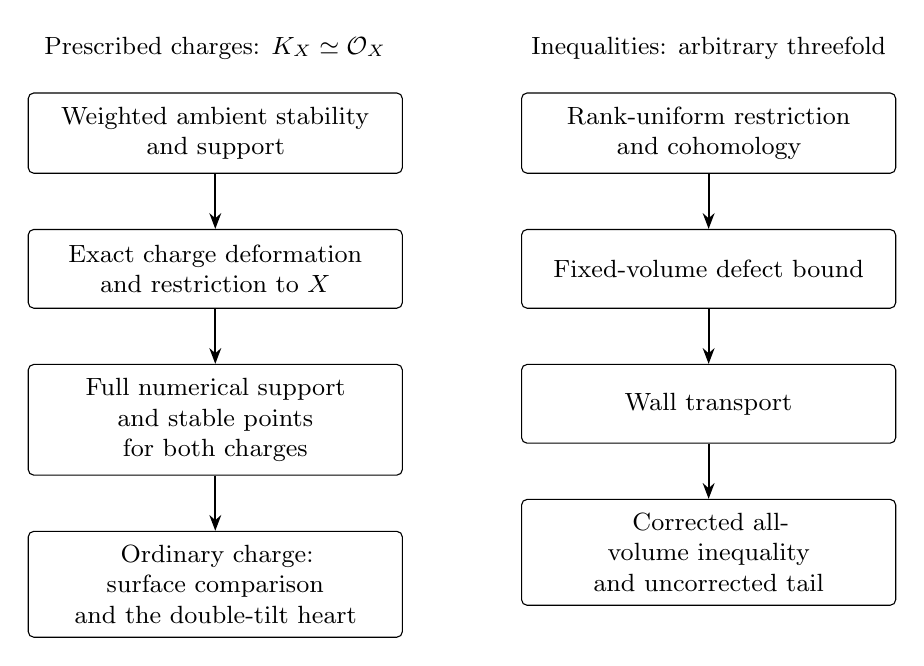
\begin{tikzpicture}[
 box/.style={draw,rounded corners=2pt,align=center,font=\small,
             text width=4.4cm,minimum height=10mm,inner sep=5pt},
 arrow/.style={-{Stealth[length=2mm]},thick}]
\node[box] (ambient) {Weighted ambient stability\\and support};
\node[box,below=7mm of ambient] (deform) {Exact charge deformation\\and restriction to $X$};
\node[box,below=7mm of deform] (support) {Full numerical support\\and stable points for both charges};
\node[box,below=7mm of support] (heart) {Ordinary charge: surface comparison\\and the double-tilt heart};
\node[box,right=15mm of ambient] (analysis) {Rank-uniform restriction\\and cohomology};
\node[above=3mm of ambient,align=center,font=\small] {Prescribed charges: $K_X\simeq\OO_X$};
\node[above=3mm of analysis,align=center,font=\small] {Inequalities: arbitrary threefold};
\node[box,below=7mm of analysis] (apex) {Fixed-volume defect bound};
\node[box,below=7mm of apex] (wall) {Wall transport};
\node[box,below=7mm of wall] (bounds) {Corrected all-volume inequality\\and uncorrected tail};
\draw[arrow] (ambient)--(deform);
\draw[arrow] (deform)--(support);
\draw[arrow] (support)--(heart);
\draw[arrow] (analysis)--(apex);
\draw[arrow] (apex)--(wall);
\draw[arrow] (wall)--(bounds);
\end{tikzpicture}
\caption{The independent categorical and numerical arguments. Full support
is obtained in Section~\ref{sec:ambient}, before the ordinary-heart
comparison in Section~\ref{sec:heart}. The numerical argument begins
with the tilt tools of Section~\ref{sec:tilt} and proves the inequalities
in Sections~\ref{sec:analysis}--\ref{sec:wall}. The relation $t=\sqrt3a$
compares volume conventions.}
\label{fig:proof}
\end{figure}

For the numerical argument, Section~\ref{sec:tilt} supplies the circle
and duality tools, Sections~\ref{sec:analysis} and~\ref{sec:apex}
establish the fixed-volume bound, and Section~\ref{sec:wall} proves
Theorem~\ref{thm:uniform-inequality} and
Corollary~\ref{cor:quadratic-tail}.
Section~\ref{sec:counterexamples} compares the inequalities with
counterexamples and bounds arbitrary-rank sheaves on reduced exceptional
surfaces.

\section{Prescribed charges on the full numerical lattice}
\label{sec:ambient}

We begin the proof of Theorem~\ref{thm:geometric-sector} by constructing
both prescribed charges with full numerical support.  This argument is
independent of the strong tilt inequalities.  Throughout the section,
$X$ is a smooth projective complex threefold with $K_X\simeq\OO_X$.

The construction takes place first on a product of projective spaces.
We choose an embedding that retains every numerical class of $X$, prove
a support estimate adapted to increasing volume on the product, and use
that estimate to deform its charge.  A fixed polynomial correction then
makes Grothendieck--Riemann--Roch restrict the deformed charge to the
chosen charge on $X$.  The same construction on smooth surface sections
will later identify the ordinary heart.
We use numerical Grothendieck groups in the Euler-pairing sense:
\[
 \Knum(X)=K_0(X)/\{v:\chi(v,u)=0\text{ for every }u\in K_0(X)\}.
\]
The left and right radicals coincide by Serre duality, so either side of
the Euler pairing may be used in the adjunction argument below.
All real vector spaces associated with these groups are finite-dimensional.
We use Bridgeland's stability conditions and locally finite slicings
\cite{Bridgeland2007}.  A stability condition has \emph{full numerical support} if, for a norm on
$\Knum(X)_\RR$, there is a constant $C$ such that
$\|[E]\|\le C|Z(E)|$ for every semistable object $E$.
The constant may depend on the stability condition.  This is equivalent to
the quadratic-form definition
\cite[Definition~1.1]{BayerDeformation2019}: one may take
$C^2|Z(v)|^2-\|v\|^2$, which is negative definite on $\ker Z$.

\subsection{An embedding which retains every numerical class}

The product-projective embedding and full-support construction here adapt
the approach of Giovenzana--Robotis--Rota--Zuliani
\cite{GiovenzanaRobotisRotaZuliani2026}.  The numerical injectivity argument
is given below; the quantitative product inputs and the prescribed-charge,
real-sector refinements are treated separately in the subsequent subsections.

\begin{lemma}\label{lem:full-numerical-embedding}
Let $X$ be a smooth projective threefold.  Rational Chern characters identify
its numerical Grothendieck group with
\begin{equation}\label{eq:full-numerical-lattice}
 \Knum(X)_\QQ\simeq
 \QQ\oplus N^1(X)_\QQ\oplus N_1(X)_\QQ\oplus\QQ.
\end{equation}
Products of numerical divisor classes span this space.  Given a real ample
class $H_*$, there are very ample line bundles $L_1,\ldots,L_q$ whose classes
form a basis of $N^1(X)_\RR$ and positive numbers $s_1,\ldots,s_q$ with
$H_*=\sum_hs_hL_h$.  For the product embedding
\begin{equation}\label{eq:product-embedding}
 i:X\hookrightarrow Y=\prod_{h=1}^q\mathbb P^{d_h},
 \qquad d_h=h^0(X,L_h)-1,
\end{equation}
the pushforward $i_*:\Knum(X)_\RR\to\Knum(Y)_\RR$ is injective.
\end{lemma}

\begin{proof}
The rational Chern character identifies the Grothendieck group with the
rational Chow group
\cite[Tags 0FDI, 0FEW, 0FB2 and 0FB5]{StacksProject}.  In Riemann--Roch the Euler pairing is the intersection
pairing after applying the invertible operations of dualizing a class and
multiplying it by $\td(X)$.  Its radical therefore gives precisely the
numerical quotient of the Chow group.  In dimensions zero and three this
quotient is $\QQ$; in the other two dimensions it is the divisor--curve
pairing in \eqref{eq:full-numerical-lattice}.

For a rational ample class $A$, the Hodge index theorem makes
$(D,D')\mapsto ADD'$ nondegenerate on $N^1(X)_\QQ$; see
\cite[Theorem~6.4 and Corollary~6.5]{GrebRossToma2016} for its
real-ample formulation.  The divisor--curve
pairing is nondegenerate by numerical equivalence, so multiplication by $A$
is an isomorphism $N^1(X)_\QQ\to N_1(X)_\QQ$.  Divisors, their products with
$A$, and $A^3$ consequently span every summand of
\eqref{eq:full-numerical-lattice}.

Choose an affine slice transverse to the ray of $H_*$ and a rational simplex
in its ample cone whose interior contains that ray.  Its $q=\rho(X)$
vertices are linearly independent.  Taking sufficiently large integral
multiples makes them very ample without changing their positive cone.  This
also explains the rank-one case, where a single very ample class suffices.

Pushforward is defined on numerical groups by adjunction with perfect
complexes.  If $i_*v=0$ numerically, the projection formula gives
\[
 \chi(i^*W,v)=\chi(W,i_*v)=0\qquad(W\in K_0(Y)).
\]
Chern characters of line bundles on $Y$ span its polynomial Chow ring, and
their restrictions span \eqref{eq:full-numerical-lattice}.  Nondegeneracy of
the Euler pairing gives $v=0$.  The spanning argument here uses dimension
three; it makes no analogous claim in arbitrary dimension.
\end{proof}

\subsection{Scaled support on elliptic products}

The next estimate is the quantitative reason that the ambient charge can
be corrected uniformly at large volume.  Its coordinates rescale a
codimension-$j$ character by the expected power $R^{n-j}$.  In these
coordinates a fixed positive-codimension correction of the exponential
charge will tend to zero as $R\to\infty$.  A support bound independent
of $R$ then turns this coordinate estimate into a bound on every
semistable object.

We first establish the support bound on an elliptic product.  The product
construction and the uniqueness needed to compare its different orders
of induction are external inputs.  The estimate below makes their volume
scaling explicit.

\begin{lemma}[Scaled support on an elliptic product]
\label{lem:elliptic-scaled-support}
Let $C$ be an elliptic curve, let $n\ge1$, and fix positive rational
numbers $\rho_1,\ldots,\rho_n$.  For rational $R\ge1$, put
$w_r=R\rho_r$ and let $H_r$ be the point-divisor class from the $r$th
factor of $C^n$.  The product stability condition with charge
\[
 Z_{\mathbf w}(u)=-\int_{C^n}e^{-i\sum_rw_rH_r}\ch(u)
\]
has support on the coordinate lattice
\[
 x_I(u)=H_I\ch_{n-|I|}(u),\qquad
 H_I=\prod_{r\in I}H_r,\qquad I\subset\{1,\ldots,n\}.
\]
More precisely, set $y_I=(\prod_{r\in I}w_r)x_I$.  In these coordinates,
\[
 Z_{\mathbf w}(u)=\widehat Z_n(y(u)),\qquad
 \widehat Z_n(y)=-\sum_I(-i)^{|I|}y_I.
\]
For a fixed Euclidean norm there is $C_n>0$, independent of $R$, such that
\[
 \|y(u)\|\le C_n|Z_{\mathbf w}(u)|
 \qquad(u\text{ the class of a semistable object}).
\]
The constants can be chosen uniformly when the positive ratios $\rho_r$
vary in a compact set.  Point sheaves are stable of phase $1$.
\end{lemma}

\begin{proof}
We use the product-with-a-curve construction of
\cite[Lemma~5.7 and Remark~5.8]{LiuProduct2021}, the positive-genus
product construction of \cite[Theorem~4.5]{ProductsCurves2025}, and
the support induction of \cite[Lemma~6.6]{LiEtAl2026}.
For $n=1$, the usual slope stability on $C$ has charge
$-x_{\varnothing}+iw_1x_{\{1\}}$ and the assertion is immediate.

Suppose that the scaled support bound has been proved in dimension
$n-1$.  Omitting factor $r$ splits the coordinates into $x',x''$,
where $x'$ consists of those containing $r$, with that index removed.
The product construction has charge
\[
 Z_{n-1}(x'')-iw_rZ_{n-1}(x').
\]
It initially gives support with respect to its own quotient lattice.
Every choice of omitted factor gives the same exponential charge and
the same phase $1$ for point sheaves.  The uniqueness theorem
\cite[Theorem~3.11]{ProductsCurves2025} therefore identifies the
slicings: that theorem permits the two support lattices to differ.
We may consequently test all the product support forms on the same
semistable objects, before proving support on the full coordinate
lattice.

Write $M_{\widehat r}$ for scaling the remaining coordinates by their
products of weights.  The scaled coordinates split as
\[
 y'=w_rM_{\widehat r}x',\qquad y''=M_{\widehat r}x''.
\]
The lower-dimensional charge in scaled coordinates is a fixed linear
map $\widehat Z$.  Increase its support constant $C_{n-1}$ if needed
and choose the support form
\begin{equation}\label{eq:elliptic-support-form}
 q_{n-1}(v)=C_{n-1}^2|\widehat Z(v)|^2-\|v\|^2.
\end{equation}
It is nonnegative on lower-dimensional semistable classes.  Crucially,
\[
 q_{n-1}(v)\le C_{n-1}^2|\widehat Z(v)|^2
 \quad\text{for every }v,
\]
not merely for semistable classes.  This is the norm form used in the
product support estimate.

For clarity, that estimate has the following coefficient condition.
Write $Z_{n-1}(x')=\alpha+i\beta$ and
$Z_{n-1}(x'')=\gamma+i\delta$.  With equal positive product parameters
$s=t=w_r$, the form
\[
 \beta\gamma-\alpha\delta
       +\eta_r q_{n-1}(M_{\widehat r}x')
\]
is nonnegative on product-semistable classes when
$0\le\eta_r\le w_r/C_{n-1}^2$
\cite[Lemma~5.7]{LiuProduct2021}; this is the substitution in
\cite[Lemma~6.6]{LiEtAl2026}.
Choose $0<\lambda_r<C_{n-1}^{-2}$, independently of $R$, and put
$\eta_r=\lambda_rw_r$.  If
\[
 \widehat Z(y')=\widehat\alpha+i\widehat\beta,
 \qquad \widehat Z(y'')=\widehat\gamma+i\widehat\delta,
\]
then multiplication of the product form by $w_r$ gives
\begin{equation}\label{eq:weighted-product-form}
 q_r(y)=\widehat\beta\widehat\gamma
       -\widehat\alpha\widehat\delta
       +\lambda_rq_{n-1}(y').
\end{equation}
All powers of $R$ have disappeared.  This form is nonnegative on the
common semistable objects just constructed.

The total charge in these coordinates is
$(\widehat\gamma+\widehat\beta)
+i(\widehat\delta-\widehat\alpha)$.  On its kernel,
\[
 q_r(y)=-|\widehat Z(y')|^2+\lambda_rq_{n-1}(y')
       =(\lambda_rC_{n-1}^2-1)|\widehat Z(y')|^2
           -\lambda_r\|y'\|^2.
\]
It is nonpositive there, and vanishes only when $y'=0$; the kernel
condition then also gives $\widehat Z(y'')=0$.
Sum \eqref{eq:weighted-product-form} over all omitted factors.  If the
sum vanishes on the total charge kernel, then $y'=0$ for every factor.
This kills every coordinate with $I\ne\varnothing$, and the charge
kills the remaining top-degree coordinate.  The summed form is thus
negative definite on the charge kernel and nonnegative on semistables.
Compactness on the unit sphere of its nonnegative cone gives
$\|y(u)\|\le C_n|Z_{\mathbf w}(u)|$ for every semistable class $u$.
The forms and all choices were made in the scaled coordinates.  In
particular they are independent of $R$ and can be kept uniform on
compact sets of positive ratios.  This completes the support induction.
The geometricity assertion is part of the positive-genus product
construction; see also \cite[Theorem~4.1(1)]{LiEtAl2026}.
\end{proof}

\subsection{Transfer to projective blocks}

For a slicing $\mathcal R$, denote the largest and smallest
Harder--Narasimhan phases of a nonzero object by $\phi^+_{\mathcal R}$ and
$\phi^-_{\mathcal R}$.  We use the distance
\[
 d(\mathcal R,\mathcal R')=
 \sup_{E\ne0}\max\{
 |\phi^+_{\mathcal R}(E)-\phi^+_{\mathcal R'}(E)|,
 |\phi^-_{\mathcal R}(E)-\phi^-_{\mathcal R'}(E)|\}.
\]
For a line bundle $L$ and an integer $k$, we say that $\mathcal R$ has
the \emph{Bayer property} for $(L,k)$ if $F\otimes L[k]$ has all phases
at least $\phi$ whenever $F\in\mathcal R(\phi)$.
We will use both a support bound and a small phase change under each
fixed line-bundle twist.  They are inherited from an elliptic product
through finite quotients.

\begin{proposition}\label{prop:weighted-ambient}
Let $Y=\prod_{h=1}^q\mathbb P^{d_h}$, put
$\xi_h=c_1(\OO_h(1))$, and fix $s_h>0$.  There is a continuous family of
numerical stability conditions $(U_R,\mathcal R_R)$ for $R\ge1$ with
\[
 U_R(u)=-\int_Ye^{-iR\sum_hs_h\xi_h}\ch(u).
\]
All point sheaves are stable of phase $1$.  Write
$\ch(u)=\sum_{\mathbf j}u_{\mathbf j}\xi^{\mathbf j}$, where
$0\le j_h\le d_h$, and set
\begin{equation}\label{eq:ambient-scaled-coordinates}
 (M_Ru)_{\mathbf j}=
 u_{\mathbf j}\prod_h(Rs_h)^{d_h-j_h}.
\end{equation}
For a fixed Euclidean norm there is $D>0$, independent of $R$, such that
\begin{equation}\label{eq:ambient-support}
 \|M_Ru\|\le D|U_R(u)|\qquad
 (u\text{ the class of an }\mathcal R_R\text{-semistable object}).
\end{equation}
For every $\mathbf e\in\ZZ^q$,
\begin{equation}\label{eq:ambient-twist-distance}
 d(\mathcal R_R,\mathcal R_R\otimes\OO_Y(\mathbf e))
 \le\sum_h\frac{d_h|e_h|}{\pi Rs_h}.
\end{equation}
\end{proposition}

\begin{proof}
Cheng proves the two-block construction and phase estimate in
\cite[Proposition~4.3 and Remark~4.4]{Cheng2026}.  We apply the same
quotient construction block by block, using
Lemma~\ref{lem:elliptic-scaled-support} to control all coordinates
uniformly in the volume.

First take $R$ and the positive weights $s_h$ rational.  Put
$n=\sum_hd_h$ and give
each of the $d_h$ elliptic factors in block $h$ the weight
$w_r=2Rs_h$.  The lemma supplies the starting stability condition and
its scaled support bound.  Only the coordinate lattice of the elliptic
power is used here; full numerical support will follow on $Y$ from the
explicit pullback calculation below.

First apply \cite[Proposition~5.1]{LiEtAl2026} to the stability condition
just constructed on the coordinate lattice.  It supplies the descent
by $(\ZZ/2)^n$ to $(\mathbb P^1)^n$ and the Bayer property with $k=0$
for every effective line bundle $\OO(a_1,\ldots,a_n)$, with all $a_r\ge0$.
We then take the symmetric quotients one block at a time.

Here is the filtration used at a symmetric step.  For
$Q=(\mathbb P^1)^d\to\mathbb P^d$, there is a finite filtration of
$\OO_{Q\times_{\mathbb P^d}Q}$ whose successive quotients are
\[
 p_2^*\mathcal L_j^{-1}\otimes\OO_{\Gamma(g_j)},
 \qquad g_j\in S_d,\qquad
 \mathcal L_j=\OO(a_{j1},\ldots,a_{jd}),\quad a_{jr}\ge0,
\]
where $p_2$ is the second projection and $\Gamma(g_j)$ is the graph
of the permutation $g_j$
\cite[Definition~3.19 and Example~3.20(3)]{LiEtAl2026}.
At a block stage the map is $f:Q\times M\to\mathbb P^d\times M$,
where $M$ is the product of the other blocks, and its fiber square is
$(Q\times_{\mathbb P^d}Q)\times M$.
Flat pullback to this product preserves the filtration and its exact
sequences.  Its graph automorphisms are $g_j\times\operatorname{id}_M$,
and its line bundles remain pulled back from $Q$.

The finite-flat descent criterion \cite[Proposition~3.21]{LiEtAl2026}
therefore requires precisely invariance under these permutations and
the Bayer properties with $k=0$ for these effective line bundles.
Indeed, for a phase-$\phi$ object $F$, the factors of $f^*f_*F$ are
$\mathcal L_j^{-1}\otimes g_{j*}F$; the two properties put their largest
phases at most $\phi$.  On the elliptic
product, signs and permutations within each equal-weight block preserve
the charge and point phases, so the uniqueness theorem used above gives
their invariance.  Block permutations normalize the full sign group;
their invariance descends through the completed involution quotient.
For subsequent block quotients, the required properties pass to the
remaining blocks as follows
\cite[Lemma~3.9 and Remark~3.14(3)]{LiEtAl2026}.
At each quotient $f:V\to V'$, pullback computes extremal phases for the
induced slicing $\mathcal S'=f_\#\mathcal S$. If a line bundle $L$ comes
from an unquotiented block, then
\[
 \phi^-_{\mathcal S'}(F\otimes L[k])
 =\phi^-_{\mathcal S}(f^*F\otimes f^*L[k]).
\]
The Bayer property for $f^*L$ therefore descends to $L$. An automorphism
of another block commutes with $f$, so its invariance descends by the
same pullback description. Thus every remaining quotient has
the required Bayer properties and invariance, for any finite number of
blocks.

For completeness, let $g$ be the resulting map from the elliptic power to
$Y$.  Pullback satisfies
\[
 g^*\xi_h^{j_h}=2^{j_h}j_h!
       \sum_{|J_h|=j_h}H_{J_h},
 \qquad \deg g=2^n\prod_hd_h!.
\]
If $|I\cap\text{block }h|=d_h-j_h$, then the scaled $I$-coordinate of
$g^*u$ is
\begin{equation}\label{eq:block-coordinate-comparison}
 \Bigl(\prod_{r\in I}w_r\Bigr)
 H_I\ch_{n-|I|}(g^*u)
 =2^n\Bigl(\prod_hj_h!\Bigr)(M_Ru)_{\mathbf j}.
\end{equation}
The fixed multiplicities are $\prod_h\binom{d_h}{j_h}$.  Pullback is thus
injective on the complete Chern-character lattice of $Y$, with norm
comparison constants independent of $R$.  Semistability pulls back, and
$Z_{\mathbf w}(g^*u)=\deg(g)U_R(u)$.  This proves \eqref{eq:ambient-support}.

For the phase estimate, vary the real tensor parameter on each elliptic
factor successively.  The one-factor argument in the proof of
\cite[Theorem~2.4]{ChengFeyzbakhsh2026}, used in
\cite[Remark~4.4]{Cheng2026}, gives its absolute variation divided by
$\pi w_r$.  A twist $e_h\xi_h$ pulls back with coefficient $2e_h$ on the
$d_h$ factors in block $h$; its factor $2$ cancels the factor $2$ in $w_r$.
Adding the variations gives \eqref{eq:ambient-twist-distance}.
Finally the deformation and multiplication-isogeny argument in the proof of
\cite[Proposition~4.3]{Cheng2026} extends the rational-weight construction
continuously to positive real weights.  It applies factor by factor: the
scaled support forms just constructed remain fixed on compact positive
weight sets, the exponential charges vary continuously, and uniqueness on
overlapping deformation neighborhoods identifies the lifts.  The closed
support inequalities and the phase bounds persist.  This also extends $R$
to all real $R\ge1$.  Point stability in this extension follows separately
from \cite[Theorem~4.1(1)]{LiEtAl2026} on the elliptic power and preservation
of geometricity under finite pushforward
\cite[Remark~3.11]{LiEtAl2026}.  Concretely, for the finite faithfully flat
quotient $g$, the sheaf $g^*\OO_y$ has a finite filtration by point sheaves,
all stable of phase $1$.  A phase-one subobject and quotient of $\OO_y$
pull back to objects whose Jordan--H\"older factors are among these points,
so both pullbacks are coherent finite-length sheaves.  Faithful flatness
descends this cohomological concentration.  The original subobject and
quotient are therefore sheaves, and simplicity of $\OO_y$ rules out a
proper nonzero subobject.  Continuity and the charge value $-1$ normalize
the point phase to $1$.
\end{proof}

\subsection{Geometric slicings and the restriction criterion}

We now prepare the restriction step.  The first consequence of point
stability below gives the cohomological bounds needed for a truncated
resolution.  The second will keep points stable during deformation in
all ambient charges.  Both will also be used to identify the induced
heart.  Write
$\mathcal R(I)$ for the extension-closed category generated by semistable
objects with phases in an interval $I$.

\begin{lemma}[Cohomological bounds from points]\label{lem:geometric-range}
Let $V$ be a smooth projective variety of dimension $n\ge2$, and let
$\mathcal R$ be a locally finite slicing in which every point sheaf is
stable of phase $1$.  Then
\begin{align}
 \mathcal R(0,1]&\subset D^{[-n+1,0]}(V),
 &\Coh(V)&\subset\mathcal R(1-n,1],\label{eq:geometric-range}\\
 D^{\le-n}(V)&\subset\mathcal R(>0),
 &\mathcal R(>0)&\subset D^{\le0}(V).\label{eq:geometric-aisles}
\end{align}
The sheaf $\mathcal H^{-n+1}(E)$ is torsion-free for
$E\in\mathcal R(0,1]$.  Moreover, $\mathcal H^0(E)$ is zero-dimensional
for $E\in\mathcal R(1)$.
\end{lemma}

\begin{proof}
This is the point-object argument of \cite[Lemma~10.1]{BridgelandK3}; we
include it to specify the dimension and boundary statements being used.
Let $E$ be stable with phase $0<\phi\le1$ and not a point of phase $1$.
Phase vanishing gives $\Hom(E,\OO_x[j])=0$ for $j<0$.
For $j\ge n$, Serre duality identifies this space with
$\Hom(\OO_x,E[n-j])^*$, which is zero by phases.  At $j=n,\phi=1$, use
nonisomorphism of the two stable objects.  The canonical bundle causes no
change, since its restriction to a point is trivial.  A minimal free
complex at each closed point consequently has nonzero terms only in
degrees $[-n+1,0]$.  Its bottom cohomology is a subsheaf of a locally free
sheaf and hence is torsion-free.  At phase $1$ we also have
$\Hom(E,\OO_x)=0$ for every $x$, so $\mathcal H^0(E)=0$.
Point sheaves themselves satisfy the stated cohomological bounds.  Finite
Jordan--Hölder filtrations and extensions give these assertions for the whole
heart; in phase $1$ its zeroth cohomology is an extension of sheaves supported
at finitely many points.

A coherent sheaf cannot receive a nonzero morphism from an object whose
phase is greater than $1$, by the cohomological bound just proved and a
shift.  It cannot map nontrivially to an object of phase at most $1-n$:
such an object is in $D^{\ge1}$, including the endpoint by the phase-one
observation.  Applied to its extreme Harder--Narasimhan factors, these
vanishings prove $\Coh(V)\subset\mathcal R(1-n,1]$.  Shifting this
inclusion and the heart bound proves \eqref{eq:geometric-aisles}.
\end{proof}

\begin{lemma}[Stability from an open set of charges]\label{lem:primitive-point}
Let a stability condition have support on a finite-rank lattice $\Lambda$.
Suppose that an object $E$ has primitive class in $\Lambda$ and remains
semistable throughout a neighborhood which is open in all central charges
$\Hom(\Lambda,\CC)$.  Then $E$ is stable.
\end{lemma}

\begin{proof}
If $E$ is strictly semistable, take a first stable subobject $G$ in a finite
Jordan--Hölder filtration.  Its class cannot be real proportional to $[E]$.
Indeed their aligned charges would make $[G]=c[E]$ with $0<c<1$, whereas
primitivity makes an integral class on this line an integral multiple of
$[E]$.  Choose a phase-window heart of length one centered at their common
phase.  The triangle $G\to E\to E/G$ remains a short exact sequence in
this heart for small deformations: all three objects stay strictly inside
its phase window.  An independent small perturbation of the two charge
values makes the phase of $G$ greater than that of $E$.  This contradicts
the assumed semistability of $E$ in the entire neighborhood.
\end{proof}

Here is the precise restriction input.  Let $f:V\to Y$ be a finite map.
For the truncated cofiltrations used below, the data consist of a finite
tower in $\Db(Y)$
\[
 E_0=f_*\OO_V\longrightarrow E_1\longrightarrow\cdots
      \longrightarrow E_N
\]
and distinguished triangles
\[
 P_j\longrightarrow E_j\longrightarrow E_{j+1}
      \longrightarrow P_j[1],\qquad 0\le j<N.
\]
Each $P_j$ is a finite direct sum of specified line bundles with specified
shifts $L_i[k_i]$, and the remainder satisfies $E_N\in D^{\le-N}(Y)$.
Thus the successive cones of the tower are $P_j[1]$; equivalently,
$f_*\OO_V$ is built by extensions from the $P_j$ and the remainder.
For a truncated resolution, $P_j$ is its $j$th sheaf term shifted by $[j]$
and $E_N$ is the last kernel shifted by $[N]$.
The finite-map restriction
criterion \cite[Proposition~3.24]{LiEtAl2026}, extending
\cite[Corollary~2.2.2]{Polishchuk2007}, applies to $f$ with this
cofiltration.  It requires
\begin{equation}\label{eq:restriction-hypotheses}
 \begin{gathered}
 \text{the Bayer properties for every }(L_i,k_i),\\
 D^{\le n_1}(Y)\subset\mathcal R(>0)\subset D^{\le n_2}(Y),
 \qquad N\ge n_2-n_1+1.
 \end{gathered}
\end{equation}
An untruncated cofiltration has no last numerical requirement.  All tensor
products in this criterion are derived.  The conclusion is a slicing
\begin{equation}\label{eq:induced-slicing}
 f^\sharp\mathcal R(\phi)=
       \{F\in\Db(V):f_*F\in\mathcal R(\phi)\},
\end{equation}
with charge $U\circ f_*$ and support on the ambient lattice through $f_*$.
In particular it provides the required Harder--Narasimhan filtrations.
No surjectivity assumption is imposed on $f$.  Smoothness makes the bounded
finite-Tor-dimension formulation applicable here.  We shall verify the
cofiltration and every bound in \eqref{eq:restriction-hypotheses} before
using the criterion.

\subsection{Correcting the charge before restriction}

Fix real classes $B_*,H_*$ with $H_*$ ample, and choose the embedding in
Lemma~\ref{lem:full-numerical-embedding}.  We write $L_h$ also for its first
Chern class, so $i^*\xi_h=L_h$ and $H_*=\sum_hs_hL_h$ with $s_h>0$.
Consider separately the factors
\begin{equation}\label{eq:two-character-factors}
 \Theta=1\qquad\text{and}\qquad
 \Theta=\sqrt{\td(X)}=1+\frac{c_2(X)}{24}.
\end{equation}
The assumption on the canonical bundle gives
$\td(X)=1+c_2(X)/12$ in the degrees relevant on $X$.  By
Lemma~\ref{lem:full-numerical-embedding}, choose a degree-two polynomial
$\delta$ in the $\xi_h$ with $i^*\delta=c_2(X)$ numerically.  A suitable
polynomial on $Y$ with constant term one is
\[
 \gamma=\begin{cases}
 \td(Y)(1-\delta/12),&\Theta=1,\\
 \td(Y)(1-\delta/24),&\Theta=\sqrt{\td(X)}.
 \end{cases}
\]
Products are taken in the finite-dimensional numerical Chow ring.  Thus
\begin{equation}\label{eq:gamma-lift}
 i^*\bigl(\gamma/\td(Y)\bigr)\td(X)=\Theta.
\end{equation}
In particular the two choices remove different Todd contributions.

Write $B=\sum_hb_hL_h$ and $H=\sum_h\ell_hL_h$.  Deform the ambient charge
to
\begin{equation}\label{eq:deformed-ambient-charge}
 U_t^{B,H}(u)=-\int_Y
 e^{-\sum_hb_h\xi_h-it\sum_h\ell_h\xi_h}\ch(u)\gamma.
\end{equation}
Grothendieck--Riemann--Roch and \eqref{eq:gamma-lift} give the exact identity
\begin{equation}\label{eq:exact-restricted-charge}
 U_t^{B,H}(i_*E)=-\int_Xe^{-B-itH}\ch(E)\Theta.
\end{equation}
Numerical equality in \eqref{eq:gamma-lift} suffices because only
intersection degrees occur.  For $\Theta=1$ this is exactly $Z_{B,tH}$;
for the other choice it is exactly $Z^{\mathrm{LV}}_{B,tH}$.

\begin{lemma}\label{lem:uniform-ambient-deformation}
For every $0<\epsilon<1/8$, there are open neighborhoods $V\ni B_*$ and
$W\ni H_*$ in the real divisor and ample spaces, and $T\ge1$, such that for all
$B\in V$, $H\in W$, and $t\ge T$, the charge
\eqref{eq:deformed-ambient-charge} lifts to a stability condition with
slicing at distance less than $\epsilon$ from
$\mathcal R_t$.  The construction is available in an open neighborhood of
that charge in the full space $\Hom(\Knum(Y),\CC)$.
\end{lemma}

\begin{proof}
Take $V$ bounded in the $b_h$ coordinates, and restrict $W$ by
$|\ell_h/s_h-1|<\eta$.  In the scaled coordinates
\eqref{eq:ambient-scaled-coordinates}, expansion of the two exponentials
gives
\begin{equation}\label{eq:uniform-deformation-estimate}
 \bigl\|(U_t^{B,H}-U_t)\circ M_t^{-1}\bigr\|
       \le C_1\eta+C_2t^{-1}.
\end{equation}
To see the uniformity, the coefficient of $u_{\mathbf j}$ in the
uncorrected exponential has degree $n-|\mathbf j|$ in $t$.  Varying the
positive coefficients $s_h$ to $\ell_h$ changes its ratio to the weight of
$M_t$ by $O(\eta)$.  A codimension-$d>0$ term of
$e^{-\sum b_h\xi_h}\gamma-1$ lowers that degree by $d$ and hence contributes
$O(t^{-d})$.  There are finitely many monomials, and their coefficients are
bounded on the chosen neighborhoods.  This proves
\eqref{eq:uniform-deformation-estimate} independently of the object.

Combine it with \eqref{eq:ambient-support}.  Choose $\eta$ first and then
$T$ so that
\[
 D(C_1\eta+C_2/T)<\sin(\pi\epsilon).
\]
To check the support hypothesis of the deformation theorem explicitly, put
\[
 Q_t(u)=D^2|U_t(u)|^2-\|M_tu\|^2.
\]
It is nonnegative on the original semistable classes.  If $U'(u)=0$ and
$\|(U'-U_t)M_t^{-1}\|\le\delta<1/D$, then
\[
 Q_t(u)\le(D^2\delta^2-1)\|M_tu\|^2<0\qquad(u\ne0).
\]
Thus $Q_t$ is negative definite on every charge kernel along the straight
deformation, and throughout the indicated open charge region.
The support-property deformation theorem
\cite[Theorem~1.2]{BayerDeformation2019} lifts the straight path while
preserving $Q_t$.  On its nonnegative cone,
$\|M_tu\|\le D|U_t(u)|$, so the relative charge change is less than
$\sin(\pi\epsilon)$.  The quantitative phase estimate
\cite[Lemma~2.9]{BayerDeformation2019} then makes the slicing distance
less than $\epsilon$ as long as it is less than $1/4$.  It is zero at the start;
continuity along the path and $\epsilon<1/8$ prevent a first exit from
that $1/4$ neighborhood.  This proves the asserted strict distance bound.
The charge bound is strict, so for each fixed $t$ it also holds on an open
neighborhood in \emph{all} ambient numerical charges.  This is the space
on which we deform, before applying restriction.
\end{proof}

\begin{proposition}\label{prop:geometric-prescribed-charges}
For either factor in \eqref{eq:two-character-factors}, the choices in
Lemma~\ref{lem:uniform-ambient-deformation} can be made so that every
$B\in V,H\in W,t\ge T$ gives a locally finite geometric stability
condition on $X$, with charge \eqref{eq:exact-restricted-charge} and full
numerical support.  Every point sheaf is stable of phase $1$.
For $\Theta=1$, the construction also gives compatible geometric slicings
on every smooth section $S_h\in|L_h|$, with Harder--Narasimhan phases
computed by pushforward to $Y$.
\end{proposition}

\begin{proof}
Set $A=\OO_Y(1,\ldots,1)$. Choose a locally free resolution
$P^\bullet\to i_*\OO_X$ with $P^0=\OO_Y$ and with each $P^{-k}$ a
finite sum of line bundles $A^{-b}$ for $k\ge1$. Such a resolution is
obtained by repeatedly generating the successive coherent kernels after
sufficiently positive twists. Fix $N>\dim Y+1$ and truncate after the
terms in degrees $0,\ldots,-(N-1)$. The remaining kernel is shifted by
$[N]$, so the cofiltration remainder lies in $D^{\le-N}(Y)$.

For a defining ambient linear form of a smooth section $S_h$, first form
the cone of the untruncated map
$P^\bullet(-\xi_h)\to P^\bullet$. It resolves
$(i\circ j_h)_*\OO_{S_h}$, and its term in degree $-k$ is
\[
 P^{-k}\oplus P^{1-k}(-\xi_h),\qquad P^1=0.
\]
Truncate each cone resolution after its terms in degrees
$0,\ldots,-(N-1)$. Its remaining kernel is again shifted by $[N]$, so
its cofiltration remainder also lies in $D^{\le-N}(Y)$.
The line bundles in all these terms are independent of the chosen smooth
section. Include all their summands, in particular the mixed twists
$A^{-b}\otimes\OO_Y(-\xi_h)$, together with $A$ and $\OO_Y(\xi_h)$,
in one finite list. This list is fixed before the parameters $B,H,t$ and
the sections are chosen.

Let $\mathcal R$ be a lift from
Lemma~\ref{lem:uniform-ambient-deformation}.  Tensoring is an isometry for
slicing distance, so \eqref{eq:ambient-twist-distance} gives, after
increasing the single threshold $T$,
\begin{equation}\label{eq:deformed-twist-distance}
 d(\mathcal R,\mathcal R\otimes L)<1
\end{equation}
for every line bundle $L$ in the finite list, uniformly in the claimed
sector.  The triangle inequality bounds the left side by
$2\epsilon+O(t^{-1})$.  The same strict inequalities hold in a full open
neighborhood of each lifted charge.

In particular tensoring by $A^{-1}[1]$ has the Bayer property.
\cite[Proposition~3.27]{LiEtAl2026} makes every point sheaf on $Y$
semistable throughout that open neighborhood.  Its numerical class is
primitive, because $\chi(\OO_Y,\OO_y)=1$.
Lemma~\ref{lem:primitive-point} upgrades semistability to stability.
At the charge \eqref{eq:deformed-ambient-charge} its value is $-1$, and
closeness to $\mathcal R_t$ fixes its phase to be $1$.

We can now apply Lemma~\ref{lem:geometric-range} on $Y$.
It supplies \eqref{eq:restriction-hypotheses} with
$n_1=-\dim Y$ and $n_2=0$.  Each resolution term $L[k]$, $k\ge1$, has
the Bayer property: \eqref{eq:deformed-twist-distance} says that tensoring
by $L$ lowers no extremal phase by as much as one, and the shift $[k]$
restores the required lower bound.  The initial $\OO_Y$ term is the
identity.  The chosen $N$ exceeds the truncation bound.  Thus the
finite-map criterion applies to the closed immersion $i$ and, when needed,
to every $i\circ j_h$.  It supplies slicings with the indicated charges
and Harder--Narasimhan filtrations.  Definition
\eqref{eq:induced-slicing} and uniqueness of those filtrations show that
pushforward computes their extremal phases.

Pushforward is exact for these hearts and detects zero objects.  A proper
destabilizing subobject of a point would therefore give one for the stable
point on $Y$.  The induced points are stable of phase $1$.
If $E$ is semistable on $X$, the ambient support inequality and the
injectivity in Lemma~\ref{lem:full-numerical-embedding} give
\[
 \|[E]\|\le C\|i_*[E]\|\le C'|U_t^{B,H}(i_*E)|.
\]
This is support on the full Euler numerical group of $X$.  For each
auxiliary surface the ambient lattice through pushforward suffices; no
injectivity assertion for its full numerical group is needed.
Finally the support bound on a finite-rank lattice gives local finiteness:
in a sufficiently short phase interval, the projection of a nonzero
semistable charge onto its middle ray has a fixed positive lower bound.
Additivity of this projection bounds the length of any chain of strict
subobjects or quotients of a fixed object in that interval.  The induced
slicings are thus locally finite, as asserted.
\end{proof}

Apply the construction to both choices of $\Theta$, intersect the two
neighborhoods $V$ and $W$, and take the larger of their thresholds.  The
same real sector and one threshold therefore work for both charges.
The proposition completes the prescribed Todd-charge assertion of
Theorem~\ref{thm:geometric-sector}.  It also supplies the exact ordinary
charge and full numerical support.  Identifying its heart requires the
additional argument in the next section.  Only $K_X\simeq\OO_X$ has been
used; no vanishing of $H^1(X,\OO_X)$ or $H^2(X,\OO_X)$ is required.

\section{The ordinary double tilt throughout the real sector}
\label{sec:heart}

For the factor $\Theta=1$, we now identify the heart furnished by
Proposition~\ref{prop:geometric-prescribed-charges}.  The method of comparing
hearts through smooth surface sections follows Cheng--Feyzbakhsh
\cite[Section~3]{ChengFeyzbakhsh2026}.  Here the charge has already been
corrected to the ordinary Chern character, and positive weighted sections
allow the polarization to be real.  The argument below proves the phase
boundaries directly.

Fix $B\in V,H\in W,t\ge T$ from the preceding construction.  Let
$\mathcal P$ be the induced slicing on $X$, with charge $Z_{B,tH}$, and put
$\mathcal C=\mathcal P(0,1]$.  As before,
$H=\sum_h\ell_hL_h$ with every $\ell_h>0$.  All restrictions of complexes
in this section are derived restrictions.

\subsection{The geometric heart on a surface}

\begin{lemma}\label{lem:surface-geometric-heart}
Let $S$ be a smooth projective surface and $(Z,\mathcal R)$ a locally finite
geometric stability condition, normalized so that point sheaves have phase
$1$.  Suppose
\[
 \Im Z(G)=\omega\bigl(c_1(G)-\beta\rk(G)\bigr),
\]
where $\omega$ is a real ample divisor class and $\beta$ a real divisor
class.  Then
\[
 \mathcal R(0,1]=\langle\mathcal F_{\omega,\beta}[1],
                              \mathcal T_{\omega,\beta}\rangle,
\]
where $\mathcal T_{\omega,\beta}$ has strictly positive slope factors
(including torsion) and $\mathcal F_{\omega,\beta}$ has nonpositive
slope factors.
\end{lemma}

\begin{proof}
Lemma~\ref{lem:geometric-range} gives
$\mathcal R(0,1]\subset D^{[-1,0]}(S)$ and
$\Coh(S)\subset\mathcal R(-1,1]$.  The comparison of these two bounded
$t$-structures makes $\mathcal R(0,1]$ a tilt of $\Coh(S)$, with torsion
pair
\[
 \mathcal T_0=\Coh(S)\cap\mathcal R(0,1],\qquad
 \mathcal F_0=\Coh(S)\cap\mathcal R(-1,0].
\]
For instance their torsion sequence is obtained by truncating a sheaf at
phase $0$; the cohomological range ensures that both pieces are sheaves.

If $G\in\mathcal T_0$, every quotient sheaf also belongs to
$\mathcal T_0$ and has nonnegative imaginary charge.  A nonzero
positive-rank quotient cannot have imaginary charge zero: it would lie in
$\mathcal R(1)$, whereas Lemma~\ref{lem:geometric-range} makes its zeroth
cohomology zero-dimensional.  Thus all positive-rank quotients of $G$ have
strictly positive slope.  Applying this to its last slope
Harder--Narasimhan quotient proves
$\mathcal T_0\subset\mathcal T_{\omega,\beta}$.
If $F\in\mathcal F_0$, then $F[1]\in\mathcal R(0,1]$, so $F$ is
torsion-free by the same lemma.  Every subsheaf remains in $\mathcal F_0$
and has nonpositive imaginary charge.  Its maximal-slope factor therefore
has slope at most zero, giving
$\mathcal F_0\subset\mathcal F_{\omega,\beta}$.

These inclusions identify the torsion pairs.  Indeed the torsion sequence
for either pair, applied to an object in the corresponding part of the
other, leaves a quotient or subobject in the intersection of its two
orthogonal parts, hence zero.  This proof includes slope zero; it does not
use a generic-parameter argument.
\end{proof}

Take a smooth section $j_h:S_h\hookrightarrow X$ in $|L_h|$ and its
compatible slicing $\mathcal P_h$.  Grothendieck--Riemann--Roch for this
divisor embedding, whose normal line bundle is $L_h|_{S_h}$, gives
\begin{equation}\label{eq:surface-induced-charge}
 Z_h(G)=-\int_{S_h}e^{-B|_{S_h}-itH|_{S_h}}\ch(G)
             \frac{1-e^{-L_h|_{S_h}}}{L_h|_{S_h}}.
\end{equation}
Since $(1-e^{-L})/L=1-L/2+L^2/6$ on a surface, its imaginary part is
\begin{equation}\label{eq:surface-imaginary-charge}
 \Im Z_h(G)=tH|_{S_h}\bigl(c_1(G)
             -(B|_{S_h}+L_h|_{S_h}/2)\rk(G)\bigr).
\end{equation}
Lemma~\ref{lem:surface-geometric-heart} identifies
\begin{equation}\label{eq:section-surface-heart}
 \mathcal P_h(0,1]=\langle\mathcal F_h[1],\mathcal T_h\rangle,
\end{equation}
where the surface slope uses $H|_{S_h}$ and twist
$B|_{S_h}+L_h|_{S_h}/2$.  Only the imaginary part of the induced charge
is needed for this identification; its real part need not be the
ordinary surface charge.

\subsection{Weighted sections give strict slope bounds}

The section-phase comparison of
\cite[Lemma~3.1]{ChengFeyzbakhsh2026} applies using the line-twist
estimate \eqref{eq:deformed-twist-distance}. The two section triangles give, for every nonzero restricted object,
\begin{align}
 \phi^-_{\mathcal P_h}(E|_{S_h})
       &\ge\phi^-_{\mathcal P}(E),\label{eq:section-lower-phase}\\
 \phi^+_{\mathcal P_h}(E(L_h)|_{S_h})
       &\le\phi^+_{\mathcal P}(E)+1.\label{eq:section-upper-phase}
\end{align}
To verify the first inequality, push the triangle
$E(-L_h)\to E\to j_{h,*}(E|_{S_h})$ to $Y$.
Its last term is an extension of $E$ and $E(-L_h)[1]$, and the latter
has smallest phase at least that of $E$ by the strict twist-distance bound.
For the second, $j_{h,*}(E(L_h)|_{S_h})$ is an extension of $E(L_h)$ and
$E[1]$, both of largest phase at most $\phi^+_{\mathcal P}(E)+1$.
Pushforward computes the induced phases, proving the assertions.

For a positive-rank sheaf, use the unnormalized slope
\[
 m_{H,B}(F)=\frac{H^2(c_1(F)-B\rk F)}{\rk F};
\]
its signs agree with the normalized slopes defining
$\mathcal B_{H,B}$.  Superscripts $+$ and $-$ denote the largest and
smallest Harder--Narasimhan slopes, with torsion assigned slope $+\infty$.
The next estimate adapts the argument of
\cite[Proposition~3.3]{ChengFeyzbakhsh2026}
by combining the sections with positive real weights. Put
\begin{equation}\label{eq:weighted-slope-gap}
 c=\frac12\sum_h\ell_hHL_h^2>0.
\end{equation}

\begin{lemma}\label{lem:heart-cohomology-slopes}
Every $E\in\mathcal C$ has cohomology in degrees $[-2,0]$, its sheaf
$\mathcal H^{-2}(E)$ is torsion-free, and
\begin{equation}\label{eq:heart-sign-bounds}
 m^+_{H,B}(\mathcal H^{-2}(E))\le-c,
 \qquad m^-_{H,B}(\mathcal H^0(E))>c.
\end{equation}
A bound for a zero sheaf is vacuous.
\end{lemma}

\begin{proof}
The range and torsion-freeness follow from
Lemma~\ref{lem:geometric-range}.  Write $F=\mathcal H^{-2}(E)$ and
$G=\mathcal H^0(E)$.  For each $h$, choose a general smooth $S_h$ which
is a nonzerodivisor on the finitely many cohomology sheaves and the
subobjects and quotients used below.  Those sheaves and sequences then
restrict without Tor.  Such choices are available inside the complete
very ample linear system.

By \eqref{eq:section-upper-phase}, $E(L_h)|_{S_h}$ has largest phase at
most $2$.  The surface tilt \eqref{eq:section-surface-heart}, applied to
its lowest ordinary cohomology, implies
$F(L_h)|_{S_h}\in\mathcal F_h$.  Similarly
\eqref{eq:section-lower-phase} places $E|_{S_h}$ in
$\mathcal P_h(>0)$, and the highest ordinary cohomology of the surface
tilt gives $G|_{S_h}\in\mathcal T_h$.  These conclusions can also be
read directly from the aisles: $\mathcal P_h(\le2)$ has its degree $-2$
cohomology in $\mathcal F_h$, while $\mathcal P_h(>0)$ has its degree
$0$ cohomology in $\mathcal T_h$.

If $F\ne0$, restrict its maximal-slope subsheaf $F'\subset F$.
The class $\mathcal F_h$ is closed under subsheaves, so the shifted twist
in the definition of the surface slope gives
\[
 \frac{HL_h(c_1(F')-B\rk F')}{\rk F'}
       \le-\frac12HL_h^2.
\]
If $G$ has a positive-rank last slope quotient $G''$, quotient-closure of
$\mathcal T_h$ gives
\[
 \frac{HL_h(c_1(G'')-B\rk G'')}{\rk G''}
       >\frac12HL_h^2.
\]
For a torsion sheaf $G$ its minimum slope is $+\infty$ instead.
Multiply the displayed inequalities by the positive $\ell_h$ and sum.
Since $\sum_h\ell_hL_h=H$, they are exactly
\eqref{eq:heart-sign-bounds}.  Positivity of the weights is what permits
this argument for a real ample $H$.
\end{proof}

\subsection{Comparison with the first tilt}

Write $\mathcal B=\mathcal B_{H,B}$ for the ordinary first tilt.  The slope
bounds just obtained place it between two adjacent translates of the
constructed heart.

\begin{lemma}\label{lem:first-tilt-phase-range}
We have
\begin{equation}\label{eq:first-tilt-phase-range}
 \mathcal B\subset\mathcal P(-1,1].
\end{equation}
Consequently
\[
 \mathcal T_0=\mathcal B\cap\mathcal P(0,1],\qquad
 \mathcal F_0=\mathcal B\cap\mathcal P(-1,0]
\]
is a torsion pair in $\mathcal B$, and
$\mathcal C=\langle\mathcal F_0[1],\mathcal T_0\rangle$.
\end{lemma}

\begin{proof}
Let $D\in\mathcal T_{H,B}$ be a sheaf with $m^-_{H,B}(D)>0$.
Lemma~\ref{lem:geometric-range} places all its phases in $(-2,1]$.
If a last Harder--Narasimhan factor $G$ had phase in $(-2,-1]$, then
$G[2]\in\mathcal P(0,1]$.  It follows that $G\in D^{[0,2]}$ and
$m^+_{H,B}(\mathcal H^0(G))\le-c$.  The canonical nonzero map $D\to G$
is tested on its degree-zero cohomology:
\[
 \Hom(D,G)=\Hom(D,\mathcal H^0(G))=0.
\]
Here the equality follows from $G\in D^{\ge0}$ and standard truncation;
the vanishing is the slope comparison, including the case of torsion $D$
since the target is torsion-free.  This contradiction excludes that phase
interval and gives $D\in\mathcal P(-1,1]$.

Now let $J\in\mathcal F_{H,B}$, so $J$ is torsion-free with
$m^+_{H,B}(J)\le0$.  The coherent-sheaf range gives
$J[1]\in\mathcal P(-1,2]$.  If a first Harder--Narasimhan factor $G$
had phase in $(1,2]$, then $G[-1]\in\mathcal P(0,1]$,
$G\in D^{[-3,-1]}$, and
$m^-_{H,B}(\mathcal H^{-1}(G))>c$.
The canonical nonzero map $G\to J[1]$ is tested on its top cohomology:
\[
 \Hom(G,J[1])=\Hom(\mathcal H^{-1}(G),J)=0,
\]
again by truncation and slope.  Thus $J[1]\in\mathcal P(-1,1]$.
Extensions prove \eqref{eq:first-tilt-phase-range}.

The final assertion is the comparison theorem for two bounded hearts one
of which lies in two adjacent degrees of the other.  Explicitly, truncate
an object of $\mathcal B$ at phase $0$ in $\mathcal P$.
The inclusion \eqref{eq:first-tilt-phase-range} and its corresponding
inclusions of aisles make both truncations objects of $\mathcal B$;
they give its torsion sequence with the two stated intersections.
Tilting that sequence recovers $\mathcal P(0,1]$.
\end{proof}

\subsection{The real-axis boundary and the second tilt}

The constructed heart is now a tilt of $\mathcal B$.  It remains to
identify the torsion pair, including the distinction between positive
and zero second slope.  The following observation, following the boundary argument of
\cite[Lemma~3.6]{ChengFeyzbakhsh2026}, controls precisely those objects.

\begin{lemma}\label{lem:phase-one-first-tilt}
An object of $\mathcal B\cap\mathcal P(1)$ is a zero-dimensional sheaf.
\end{lemma}

\begin{proof}
Let $E$ belong to the stated intersection.  Its ordinary cohomology is
$J=\mathcal H^{-1}(E)\in\mathcal F_{H,B}$ and
$U=\mathcal H^0(E)\in\mathcal T_{H,B}$.
Lemma~\ref{lem:geometric-range} makes $U$ zero-dimensional.
Choose the smooth sections $S_h$ to avoid its finite support and to
restrict $J$ without Tor.  If $J\ne0$, it is torsion-free of positive
rank, and $E|_{S_h}=J|_{S_h}[1]$.
Inequality \eqref{eq:section-lower-phase} gives
$\phi^-_{\mathcal P_h}(J|_{S_h})\ge0$.
Its phases as a coherent sheaf are also at most $1$, by
Lemma~\ref{lem:geometric-range}.  Hence
$\Im Z_h(J|_{S_h})\ge0$ and \eqref{eq:surface-imaginary-charge} gives
\[
 \frac{HL_h(c_1(J)-B\rk J)}{\rk J}\ge\frac12HL_h^2
 \quad\text{for each }h.
\]
The positive weighted sum says $m_{H,B}(J)\ge c>0$, contrary to
$m^+_{H,B}(J)\le0$.  Therefore $J=0$ and $E=U$.
\end{proof}

We use the physical second slope from the introduction, writing
$\nu^{\mathrm{phys}}_{B,tH}=\nu_{B,tH}$ to distinguish it from
$\nu_{a,b}$:
\begin{equation}\label{eq:physical-second-slope}
 \nu^{\mathrm{phys}}_{B,tH}(E)=
 \frac{tH\ch_2^B(E)-t^3H^3\ch_0(E)/6}
 {t^2H^2\ch_1^B(E)},
\end{equation}
with value $+\infty$ at a zero denominator.  The tilt
Harder--Narasimhan property for each fixed real ample class $tH$ and real
$B$ is the input of \cite[Section~2]{BMS2016}; here no continuity as the
ample direction varies is required.  Its Harder--Narasimhan filtration
defines the torsion pair $(\mathcal T',\mathcal F')$ in
$\mathcal B$ with strictly positive slopes in $\mathcal T'$ and
nonpositive slopes in $\mathcal F'$.  Multiplication by a positive
constant does not affect this pair.  The claimed double tilt is
$\mathcal A_{B,tH}=\langle\mathcal F'[1],\mathcal T'\rangle$.

\begin{lemma}\label{lem:physical-zero-denominator}
For $E\in\mathcal B$ the denominator in
\eqref{eq:physical-second-slope} is nonnegative.  If it vanishes, then
$\Im Z_{B,tH}(E)\ge0$, with equality only for a zero-dimensional sheaf.
\end{lemma}

\begin{proof}
Let $J=\mathcal H^{-1}(E)$ and $U=\mathcal H^0(E)$.
The first torsion pair makes each contribution to
$H^2\ch_1^B(E)=H^2\ch_1^B(U)-H^2\ch_1^B(J)$ nonnegative.
If the sum is zero, $J$, when nonzero, is slope-semistable of slope zero,
and $U$ has dimension at most one.  Indeed positive-rank quotients in the
positive torsion part have strictly positive degree, and a nonzero
effective divisorial cycle has positive intersection with $H^2$.
For real $H$, the K\"ahler Bogomolov--Gieseker inequality follows from
\cite[Theorem~1.1, Equation~(1.6)]{LiZhangZhang2017}, applied with zero
Higgs field to the reflexive hull $J^{**}$ when $J\ne0$.
This hull is semistable for the same $H$: intersecting a subsheaf of
$J^{**}$ with $J$ preserves its rank and first Chern class.
The quotient $Q=J^{**}/J$ has codimension at least two, and, writing
$r=\rk J$, additivity gives
\[
 c_1(J)^2-2r\ch_2(J)
 =c_1(J^{**})^2-2r\ch_2(J^{**})+2r\ch_2(Q),
\]
where $\ch_2(Q)$ is an effective curve cycle, so the inequality descends
to $J$.
The same argument on a surface uses an effective zero-cycle correction;
neither application changes the real polarization.
Classical Bogomolov--Gieseker and the real-ample Hodge index theorem
\cite[Theorem~6.4]{GrebRossToma2016}, applied to
$H^2\ch_1^B(J)=0$, give
$H\ch_2^B(J)\le0$.  The curve cycle of $U$ is effective.  Consequently
\[
 \Im Z_{B,tH}(E)=
 tH\ch_2^B(U)-tH\ch_2^B(J)+\frac{t^3H^3}{6}\rk J\ge0.
\]
If $J\ne0$, the last term is strictly positive.  If $J=0$ and $U$ has a
nonzero one-dimensional part, its curve degree is strictly positive.
Thus equality is possible exactly when $E=U$ is zero-dimensional.
\end{proof}

\begin{proposition}\label{prop:exact-double-tilt-heart}
For the factor $\Theta=1$ throughout the real sector of
Proposition~\ref{prop:geometric-prescribed-charges},
\[
 \mathcal P(0,1]=\mathcal A_{B,tH}.
\]
\end{proposition}

\begin{proof}
Compare $(\mathcal T',\mathcal F')$ with the torsion pair
$(\mathcal T_0,\mathcal F_0)$ of
Lemma~\ref{lem:first-tilt-phase-range}.
For $D\in\mathcal T'$, take its latter torsion sequence
$0\to D_1\to D\to D_2\to0$.
A nonzero $D_2\in\mathcal F_0$ has $\Im Z(D_2)\le0$.
Its denominator cannot vanish: Lemma~\ref{lem:physical-zero-denominator}
would make it zero-dimensional, whereas zero-dimensional sheaves are in
$\mathcal P(1)$ and $\mathcal F_0\subset\mathcal P(-1,0]$.
Thus $D_2$ has positive denominator and
$\nu^{\mathrm{phys}}_{B,tH}(D_2)\le0$, contradicting the strictly positive
slopes of every nonzero quotient of $D$.  Hence
$\mathcal T'\subset\mathcal T_0$.

For $D\in\mathcal F'$, consider $D_1$ in the same torsion sequence.
A nonzero subobject of $D$ has second slope at most zero, so $D_1$ has
positive denominator and $\Im Z(D_1)\le0$.
But $D_1\in\mathcal T_0\subset\mathcal P(0,1]$ makes its imaginary
charge nonnegative.  It must therefore vanish, and $D_1\in\mathcal P(1)$.
Lemma~\ref{lem:phase-one-first-tilt} makes it zero-dimensional, whose second
slope is $+\infty$, a contradiction.  Thus
$\mathcal F'\subset\mathcal F_0$.
The two inclusions identify the torsion pairs, and their tilts coincide.
\end{proof}

Proposition~\ref{prop:exact-double-tilt-heart}, together with
Proposition~\ref{prop:geometric-prescribed-charges}, proves the ordinary
charge assertion of Theorem~\ref{thm:geometric-sector}, including its exact
heart, full numerical support, local finiteness, stable points, and one
threshold for an open real sector.  The equality of hearts was proved only
for $\Theta=1$.  The Todd-charge construction retains its geometric heart
from the preceding section.

Finally, the coefficient in the strong inequality should be kept distinct
from the weaker sign consequence of this construction.  If $E\ne0$ is
first-tilt semistable of finite physical slope zero, then
$E[1]\in\mathcal A_{B,tH}$ and its nonzero real charge is negative.  Thus
\[
 \ch_3^B(E)<\frac{t^2}{2}H^2\ch_1^B(E).
\]
With $t=\sqrt3a$, the strong inequality has coefficient $t^2/18$ instead.
The categorical argument supplies the real-sector and full-support
conclusions; the sharper coefficient will be proved independently in
Sections~\ref{sec:apex} and~\ref{sec:wall} by the fixed-volume estimate
and wall transport.

\section{Tilt stability and numerical transport}
\label{sec:tilt}

We now begin the independent proof of
Theorem~\ref{thm:uniform-inequality}, which applies to arbitrary smooth
projective threefolds along a fixed integral ample direction.  The
inequality will first be proved at one volume, then transported to all
positive volumes.  This section supplies the tilt conventions and
deformation facts needed for that transport.  Objects with zero reduced
charge must be retained: they affect both finite factor filtrations and
duality at real parameters.

\subsection{Characters, slopes, and the first tilt}

Throughout this section, $X$ is a smooth projective complex threefold,
$H$ is an integral ample divisor class, and $h=H^3$.  All intersections
and Chern characters are numerical.  For a real divisor class $T$, set
$\ch^T(E)=e^{-T}\ch(E)$ and use the normalized coordinates
\begin{equation}\label{eq:normalized-characters}
\begin{gathered}
 r(E)=\ch_0(E),\qquad c_T(E)=\ch_1^T(E),\\
 d_T(E)=\frac{H^2c_T(E)}h,\qquad
 w_T(E)=\frac{H\ch_2^T(E)}h,\qquad
 z_T(E)=\frac{\ch_3^T(E)}h.
\end{gathered}
\end{equation}
The subscript $0$ is reserved for the untwisted character.  Fix
$B_0\in N^1(X)_{\QQ}$ and put $B=B_0+bH$ for $b\in\RR$.
We abbreviate the twist $B_0+bH$ by a symbolic subscript $b$;
when evaluating at $b=0$, we write the subscript $B_0$ explicitly.
The exponential formula gives
\begin{align}
 d_b&=d_{B_0}-br,&
 w_b&=w_{B_0}-b d_{B_0}+\tfrac12b^2r,\label{eq:twist-two}\\
 z_b&=z_{B_0}-b w_{B_0}+\tfrac12b^2d_{B_0}-\tfrac16b^3r.
 \label{eq:twist-three}
\end{align}

For a positive-rank coherent sheaf define
$\mu_{H,B}=d_B/r$, and give every nonzero torsion sheaf slope
$+\infty$.  Let $\mu^+$ and $\mu^-$ be the largest and smallest slopes
in the slope Harder--Narasimhan filtration.  The torsion pair and its tilt
are
\begin{equation}\label{eq:first-tilt}
\begin{gathered}
 \mathcal T_{H,B}=\{U:\mu^-_{H,B}(U)>0\},\qquad
 \mathcal F_{H,B}=\{V:\mu^+_{H,B}(V)\le0\},\\
 \mathcal B_{H,B}=\langle\mathcal F_{H,B}[1],\mathcal T_{H,B}\rangle,
\end{gathered}
\end{equation}
where the zero sheaf belongs to both parts.  This is the heart of a
bounded $t$-structure.  For $a>0$ put
\begin{equation}\label{eq:tilt-numerator}
 n_{a,b}=w_b-\tfrac12a^2r,\qquad
 \nu_{a,b}(E)=
 \begin{cases}n_{a,b}(E)/d_b(E),&d_b(E)>0,\\
 +\infty,&d_b(E)=0.
 \end{cases}
\end{equation}
For a general real twist $B$, the same formula defines
$\nu_{a,B}$ using $d_B,w_B$ and $n=w_B-a^2r/2$; the notation
$\nu_{a,b}$ specifies the line $B=B_0+bH$.
An object is tilt-stable, respectively tilt-semistable, if every proper
nonzero subobject $F\subset E$ in $\mathcal B_{H,B}$ satisfies
$\nu(F)<\nu(E/F)$, respectively $\nu(F)\le\nu(E/F)$.
This is the convention of \cite[Definition~2.3]{BMS2016}.
The physical parameter $\omega=\sqrt3aH$ used in
\cite{BMT2014,BMS2016} multiplies our finite slope by $1/(\sqrt3a)$,
so defines the same stable and semistable objects.

Here are two harmless reductions for the inequality.  Write
$q=H^2B_0/h$ and replace $(B_0,b)$ by $(B_0-qH,b+q)$; the twist
$B$ is unchanged, and the new rational $B_0$ satisfies $H^2B_0=0$.
If $H'=sH$ is very ample, use $a'=a/s$ and $b'=b/s$.
The hearts agree and $\nu'_{a',b'}=\nu_{a,b}/s$.  An estimate with
correction $k'(H')^2$ becomes an estimate with correction
$s^2k'H^2$, and a threshold $a'>R'$ becomes $a>sR'$.
We may therefore assume $H$ very ample and $H^2B_0=0$ while proving
the estimates.  Constants used with duality are chosen for both $B_0$
and $-B_0$.

\subsection{Discriminants and finite-slope filtrations}

The Hodge index theorem gives a useful norm on $N^1(X)_{\RR}$.
Define
\begin{equation}\label{eq:divisor-norm}
 \langle C,D\rangle=\frac{HCD}{h},\qquad
 C_\perp=C-\langle H,C\rangle H,\qquad
 \|C\|^2=\langle H,C\rangle^2-\langle C_\perp,C_\perp\rangle.
\end{equation}
The pairing is negative definite on $H^\perp$, so this is a positive
definite norm.  For a positive-rank torsion-free sheaf $G$ put
\begin{equation}\label{eq:sheaf-discriminants}
\begin{gathered}
 \mu(G)=\frac{d_0(G)}{r(G)},\qquad
 \xi_G=\left\langle\frac{c_0(G)}{r(G)},\frac{c_0(G)}{r(G)}\right\rangle
             -\frac{2w_0(G)}{r(G)},\\
 \delta_G^T=\left(\frac{d_T(G)}{r(G)}\right)^2
             -\frac{2w_T(G)}{r(G)}.
\end{gathered}
\end{equation}
Classical Bogomolov--Gieseker gives $\xi_G\ge0$ for slope-semistable
$G$.  Twist invariance of the full discriminant and the orthogonal
decomposition in \eqref{eq:divisor-norm} give
\begin{equation}\label{eq:xi-delta}
 \delta_G^T=\xi_G-\left\langle
 \left(\frac{c_0(G)}{r(G)}-T\right)_\perp,
 \left(\frac{c_0(G)}{r(G)}-T\right)_\perp\right\rangle\ge\xi_G.
\end{equation}
Slope filtrations of torsion-free sheaves may be refined to slope-stable
torsion-free factors: take saturated equal-slope subsheaves inside a
semistable factor and induct on rank.

For arbitrary derived objects the projected discriminant is
\begin{equation}\label{eq:projected-discriminant}
 \Delta(E)=d_b(E)^2-2r(E)w_b(E)
           =d_{B_0}(E)^2-2r(E)w_{B_0}(E).
\end{equation}
Its independence of $b$ follows from \eqref{eq:twist-two}.
We use the following established tilt-stability input for a \emph{fixed}
integral ample class $H$.  There are Harder--Narasimhan filtrations for
all $a>0$ and real $B$; tilt-stability is open in $(a,B)$; the extremal
phases of a fixed derived object vary continuously; and every
tilt-semistable object satisfies
\begin{equation}\label{eq:tilt-discriminants}
 \Delta\ge0,\qquad
 \langle c_B,c_B\rangle-2rw_B+C_Hd_B^2\ge0
\end{equation}
for a constant $C_H\ge0$ depending only on $X,H$.
These are \cite[Theorem~3.5 and Propositions~B.2 and~B.5]{BMS2016},
with volume factors absorbed into $C_H$.  The continuous reduced charge
is $d_B+i(w_B-a^2r/2)$, with heart phase interval
$(-1/2,1/2]$ and phase $1/2$ assigned to its zero-charge objects.
No assertion about varying the direction of $H$ is used here;
\cite[Remark~B.6(b)]{BMS2016} expressly distinguishes that question.

\begin{lemma}\label{lem:tilt-zero-denominator}
An object $E\in\mathcal B_{H,B}$ has $d_B(E)\ge0$.
Write $n=w_B-a^2r/2$.
If $d_B(E)=0$, then $n(E)\ge0$, with equality exactly when
$E$ is a zero-dimensional sheaf, including the zero object.
For a finite-slope object $E$, semistability is equivalent to the
condition that every proper nonzero subobject has positive denominator
and slope at most $\nu(E)$.  Every finite-slope quotient of a
finite-slope semistable object has slope at least $\nu(E)$.
\end{lemma}

\begin{proof}
Write $V=\mathcal H^{-1}(E)$ and $U=\mathcal H^0(E)$ for ordinary
cohomology.  The defining torsion pair gives $d_B(V)\le0$ and
$d_B(U)\ge0$, whence $d_B(E)=d_B(U)-d_B(V)\ge0$.
If it is zero, a nonzero $V$ is torsion-free and slope-semistable of
slope zero, whereas $U$ has dimension at most one.  Bogomolov--Gieseker
and Hodge index give $w_B(V)\le0$; effectiveness of the curve cycle
gives $w_B(U)\ge0$.  Thus
\[
 n(E)=w_B(U)-w_B(V)+\tfrac12a^2r(V)\ge0.
\]
Equality forces $V=0$ and the curve cycle of $U$ to vanish, so $U$ is
zero-dimensional.  The converse is immediate.

In a short exact sequence $0\to F\to E\to G\to0$ with $d(E)>0$,
a subobject with $d(F)=0$ has slope $+\infty$ while $d(G)>0$.
It is forbidden by semistability.  If both denominators are positive,
additivity makes $\nu(E)$ their weighted average, proving the desired
equivalences.  If $d(G)=0$, then $n(G)\ge0$, so
$\nu(F)\le\nu(E)$ and comparison with $\nu(G)=+\infty$ is automatic.
\end{proof}

Strict comparison with the quotient is significant: a zero-dimensional
quotient does not destroy stability in our convention, although it
gives equality between the slopes of the subobject and the object.
An object stable for the stricter subobject--object convention is
semistable in ours, and is therefore covered by all the inequalities
below.

\begin{lemma}\label{lem:tilt-support-bound}
For fixed $a>0$ there is a constant $C_a$, depending only on $a,X,H$,
such that every tilt-semistable object, at any real twist $B$, satisfies
\begin{equation}\label{eq:tilt-support-bound}
 |r|+|w_B|+\|c_B\|\le C_a(d_B+|n|),\qquad n=w_B-a^2r/2.
\end{equation}
The constants can be bounded uniformly when $a$ ranges in a compact
subinterval of $(0,\infty)$.
\end{lemma}

\begin{proof}
The first inequality of \eqref{eq:tilt-discriminants} gives
$a^2r^2+2rn\le d^2$, and hence
$|r|\le 2|n|/a^2+d/a$.  The equality $w=n+a^2r/2$ bounds $|w|$.
Finally the second inequality gives
\[
 \|c_B\|^2=2d^2-\langle c_B,c_B\rangle
 \le(2+C_H)d^2-2rw,
\]
which proves the norm bound.  These expressions also prove uniformity
on compact $a$-intervals.
\end{proof}

This estimate controls rank, the full first character, and one degree
of the second character.  It is not a support statement on the full
numerical Grothendieck group.  Its immediate use is to make a
finite-slope factorization terminate even when $b$ is irrational.

\begin{lemma}\label{lem:finite-tilt-factors}
Every nonzero finite-slope tilt-semistable object has a finite
filtration in $\mathcal B_{H,B}$ whose factors are tilt-stable of the
same finite slope.  Extensions of finite-slope semistable objects of
the same slope are semistable of that slope.
\end{lemma}

\begin{proof}
Let $\nu(E)=u\in\RR$.  If $E$ is not stable, there is a proper
nonzero subobject $F$ with $\nu(F)=\nu(E/F)=u$ and positive
denominators.  The object $F$ is semistable by
Lemma~\ref{lem:tilt-zero-denominator}.  To obtain a splitting into
two semistable objects, we may have to absorb a zero-dimensional
subobject of the quotient back into $F$.  Put $G=E/F$ and take its
Harder--Narasimhan filtration.  Its last factor is a quotient of $E$,
so, if its slope is finite, that slope is at least $u$.  The other
finite slopes are no smaller.  There must be a finite factor since
$d(G)>0$.  Additivity of $n-ud$, together with the nonnegativity of
$n$ on infinite-slope factors, now forces all finite slopes to equal
$u$ and all infinite-slope factors to have $d=n=0$.
Thus $G$ is either semistable or has a zero-dimensional initial
subobject $T$ followed by a semistable quotient of slope $u$.
Replace $F$ by the preimage of $T$.  It is still a proper
equal-slope subobject of $E$, hence semistable, and its quotient is
now semistable as well.

Repeated splitting cannot produce arbitrarily many nonzero factors.
For a semistable factor of slope $u$, Lemma~\ref{lem:tilt-support-bound}
gives $|r|\le C_a(1+|u|)d$.  If $r\ne0$, integrality of rank
therefore bounds $d$ below by $1/(C_a(1+|u|))$.
If $r=0$, then $d=H^2\ch_1/h$ is positive and belongs to
$h^{-1}\ZZ$, so $d\ge1/h$.  Each factor has denominator at least
the smaller of these two positive constants, and their denominators
sum to $d(E)$.  A finite number of splits consequently gives stable
factors.

For the extension assertion, intersect a subobject with the first
term and take its image in the last term.  A nonzero intersection or
image has positive denominator and slope at most $u$ by semistability.
Their sum has the same properties, proving the subobject criterion.
\end{proof}

\subsection{Semistability on the numerical semicircle}

The next observation brings a nonzero finite slope to slope zero.
It also supplies the side points used in the fixed-apex argument.
It extends the calculation of \cite[Lemma~4.3]{BMS2016} to a fixed
transverse twist $B_0$.

\begin{lemma}\label{lem:tilt-semicircle}
Suppose $E$ is tilt-semistable of finite slope $u$ at $(a,b)$.
Put $c=b+u$ and $R=\sqrt{a^2+u^2}$.  Then $E$ is
tilt-semistable at every point
\begin{equation}\label{eq:tilt-semicircle}
 b'=c+x,\qquad a'=\sqrt{R^2-x^2},\qquad -R<x<R,
\end{equation}
and its slope there is $-x$.  In particular it is semistable of
slope zero at $(R,c)$.
\end{lemma}

\begin{proof}
Since $w_b=ud_b+a^2r/2$, the twist formulas give
$w_c=R^2r/2$ and $d_c=d_b-ur$.  Thus
$\Delta=d_c^2-R^2r^2\ge0$.  If $r\ne0$, the negative alternative
$d_c\le-R|r|$ would give
$d_b=d_c+ur\le-(R-|u|)|r|<0$.  It follows that
$d_c\ge R|r|$; for $r=0$ we have $d_c=d_b>0$.
On the whole open arc, therefore,
\[
 d_{b'}=d_c-xr>0,\qquad
 n_{a',b'}=-x(d_c-xr).
\]

Consider the set of points on the arc where $E$ is semistable in
the corresponding heart.  It contains the original point.  It is
closed within the arc: the formal charge has positive real part,
and continuity of the largest and smallest phases makes both
converge to its finite phase.  In particular, this argument also
ensures membership in the limiting heart.
It is open within the arc as well.  At a semistable point take the
finite stable filtration from Lemma~\ref{lem:finite-tilt-factors}.
Every factor has the same slope there and thus the same $c,R$ in
\eqref{eq:tilt-semicircle}.  Openness of stability keeps all these
finitely many factors stable in nearby hearts, with their common
slope $-x$.  Their fixed triangles are short exact sequences in
those hearts, and their extensions are semistable by the preceding
lemma.  Connectedness of the arc proves the assertion.
\end{proof}

\subsection{Duality, including the point defect}

To treat negative rank we use the shifted derived dual
$\mathbb D(E)=R\mathcal Hom(E,\OO_X)[1]$.

\begin{lemma}\label{lem:tilt-duality}
Let $a>0$, let $B$ be real, and let $E\in\mathcal B_{H,B}$
be tilt-semistable of finite slope $u$.  There are a zero-dimensional
sheaf $T_0$ and a distinguished triangle
\begin{equation}\label{eq:tilt-dual-triangle}
 \widetilde E\longrightarrow\mathbb D(E)\longrightarrow T_0[-1]
 \longrightarrow\widetilde E[1],
\end{equation}
where $\widetilde E\in\mathcal B_{H,-B}$ is tilt-semistable of
slope $-u$.  At twists $B$ and $-B$ respectively their coordinates
are related by
\begin{equation}\label{eq:tilt-dual-characters}
 (r,d,w,z)(\widetilde E)
   =\bigl(-r(E),d_B(E),-w_B(E),z_B(E)+\operatorname{length}(T_0)/h\bigr).
\end{equation}
Moreover $\widetilde E=\tau^{\le0}\mathbb D(E)$ for the ordinary
cohomological truncation.
\end{lemma}

\begin{proof}
For rational $\omega=\sqrt3aH$ and rational $B$,
\cite[Proposition~5.1.3(b)]{BMT2014} gives the triangle and
semistability directly: its hypothesis is finite maximal tilt slope,
which holds for a finite-slope semistable object.  In that triangle
$\widetilde E$ has ordinary cohomology in degrees $-1,0$, whereas
$T_0[-1]$ is in degree $1$.  Hence $\widetilde E$ is the stated
ordinary truncation; it depends only on $E$.

First suppose $E$ is stable at real parameters.  By openness it is
stable at a sequence of nearby parameters with rational $\omega,B$.
The rational triangles all have the same truncation
$\tau^{\le0}\mathbb D(E)$ and the same sheaf
$\mathcal H^1(\mathbb D(E))$.  Their mirror finite phases converge
to the phase of slope $-u$, with the denominator still positive.
Continuity of extremal phases therefore gives semistability of this
fixed truncation in $\mathcal B_{H,-B}$.

For a semistable $E$, use Lemma~\ref{lem:finite-tilt-factors} and
induct on its number of stable factors.  For an extension
$0\to E_1\to E\to E_2\to0$, duality reverses the triangle.
We must show that its degree-zero cohomology in the mirror tilt heart
is semistable and that its degree-one cohomology is zero-dimensional.
The cohomology sequence is
\[
 0\longrightarrow\widetilde E_2\longrightarrow
 \mathcal H^0_{\mathcal B_{H,-B}}(\mathbb D(E))
 \longrightarrow\widetilde E_1\longrightarrow T_{0,2}
 \longrightarrow\mathcal H^1_{\mathcal B_{H,-B}}(\mathbb D(E))
 \longrightarrow T_{0,1}\longrightarrow0,
\]
and all other tilt cohomology vanishes.  Subobjects and quotients
of a zero-dimensional sheaf in this heart are zero-dimensional:
additivity first forces both denominators to vanish, then both
nonnegative numerators to vanish, and
Lemma~\ref{lem:tilt-zero-denominator} applies.
Consequently the kernel of $\widetilde E_1\to T_{0,2}$ has the
same positive denominator and the same slope as $\widetilde E_1$;
it is semistable by the subobject criterion.  The degree-zero term
is an extension of it by $\widetilde E_2$, and is semistable of
slope $-u$.  The degree-one term is zero-dimensional.  This proves
\eqref{eq:tilt-dual-triangle}, including its truncation description,
for the extension.

Finally the shifted dual has characters $(-r,c_B,-\ch_2^B,\ch_3^B)$
at twist $-B$.  The term $T_0[-1]$ has third character
$-\operatorname{length}(T_0)$, so taking characters of the triangle
gives \eqref{eq:tilt-dual-characters}.
\end{proof}

\section{Restriction and cohomology bounds}
\label{sec:analysis}

The estimates in this section convert numerical control of slope factors
into control of sections and first cohomology.  The constants depend on the
polarized variety and on specified twist ranges, but not on the ranks of
the sheaves.  This distinction is essential: the first-cohomology estimate
will be proportional to a discriminant error, which can vanish even when
the rank is large.

Throughout this section, $H$ is very ample and $h=H^3$.  On a smooth
surface $S\in|H|$, we use
\[
 d_T(G)=\frac{H|_S\,\ch_1^T(G)}h,
 \qquad w_T(G)=\frac{\ch_2^T(G)}h,
 \qquad \mu_T(G)=\frac{d_T(G)}{\rk G}.
\]
For divisor classes on $S$, put $\langle C,D\rangle=CD/h$ and use the
norm
\[
 \|C\|^2=\langle H,C\rangle^2-\langle C_\perp,C_\perp\rangle,
 \qquad C_\perp=C-\langle H,C\rangle H.
\]
Here and below $H$ also denotes its restriction.  The definitions of
$\xi_G$ and $\delta_G^T$ consequently have the same formulas as on $X$.
In particular, for a positive-rank sheaf they give the identity
\begin{equation}\label{eq:surface-norm-discriminant}
 \mu_T(G)^2+\delta_G^T
 =\left\|\frac{c_1(G)}{\rk G}-T\right\|^2+\xi_G.
\end{equation}
On a smooth curve $C_m\in|mH|_S$, normalize the slope as
$\mu(G)=\deg(G)/(mh\rk G)$.  This makes the slope of an unmodified
restriction equal to the slope before restriction.

The first-cohomology estimate will concern stable surface sheaves
whose normalized first character is close to a negative scalar class.
For the fixed rational twist $B_0$, write
\[
 T=B_0|_S+(b-A)H,\qquad |b|\le1.
\]
For sufficiently large $A$, our target is to bound first cohomology
at fixed twists by sums of
\[
 r(G)\left(\left\|\frac{c_1(G)}{r(G)}-T\right\|^2+\xi_G\right).
\]
This quantity can vanish even when the total rank is large.  The
negative scalar part of $T$ will give positive central curvature on
the dual bundle; its trace-free curvature will then control the
remaining harmonic forms.  A separate estimate for sections uses the
rank of a subsheaf's evaluation map.  We first choose surfaces and
curves with uniform geometry, so that both estimates have constants
independent of the sheaves and their ranks.

\subsection{Restriction and the choice of smooth sections}

\begin{lemma}[Restriction variance]\label{lem:restriction-variance}
Let $G$ be a slope-semistable torsion-free sheaf of rank $r>0$ on $X$.
For a very general smooth $S\in|H|$, restrict $G$ and refine its slope
Harder--Narasimhan filtration into slope-stable torsion-free factors
$G_i$, with ranks $r_i$ and normalized slopes $\mu_i$.  Then
\begin{equation}\label{eq:restriction-variance}
 \sum_i r_i\bigl(\mu_i-\mu(G)\bigr)^2\le r\xi_G.
\end{equation}
The same assertion holds for a slope-semistable torsion-free sheaf on
$S$, restricted to a very general smooth $C_m\in|mH|_S$, for every
positive integer $m$.

More generally, restrict a finite filtration with semistable
torsion-free factors and refine each restricted factor separately.
From $X$ to $S$, for any fixed divisor twist $T$ on $X$, restricted
to $S$, the increases in
$\sum_i r_i\mu_T(G_i)^2$ and in $\sum_i r_i\delta_{G_i}^T$ are equal
and lie between zero and the original sum $\sum_G r(G)\xi_G$.
From $S$ to $C_m$, the same upper bound holds for the increase of the
second slope moment, using any fixed divisor twist on $S$ and its
restriction to $C_m$.  The concatenated filtration need not be the
Harder--Narasimhan filtration of the whole restriction.
\end{lemma}

\begin{proof}
Write
\[
 \operatorname{Disc}(G)
 =2r c_2(G)-(r-1)c_1(G)^2=c_1(G)^2-2r\ch_2(G).
\]
The characteristic-zero semistable case of Langer's restriction
inequality \cite[Theorem~3.1]{Langer2004} has zero extremal-slope
term.  On $X$ it gives, for raw restricted slopes $s_i=h\mu_i$,
\[
 \sum_{i<j}r_i r_j(s_i-s_j)^2
 \le hH\operatorname{Disc}(G)=h^2r^2\xi_G.
\]
Since $\sum r_i\mu_i=r\mu(G)$, the left side is
$h^2r\sum_i r_i(\mu_i-\mu(G))^2$.
Division gives \eqref{eq:restriction-variance}.  If the restriction is
semistable, its left side is zero, and the inequality follows directly
from $\xi_G\ge0$.  Refinement at a fixed slope leaves the sum unchanged.
For a surface restriction, apply the same theorem with its very ample
divisor $mH$.  The raw slopes are $s_i=mh\mu_i$ and the right side is
$m^2h\operatorname{Disc}(G)=m^2h^2r^2\xi_G$; the factors $m^2h^2r$
cancel in the same way.

We use the corrected very-general formulation of the theorem
\cite[p.~1211]{Langer2004Addendum}.  In the ample polarizations used
here, that addendum also permits general divisors: the stated
difficulty concerns the remaining nef polarizations when they are
not ample.

For each original factor, the weighted mean of its restricted slopes
is unchanged.  Subtracting a fixed scalar $\mu(T)$ from these slopes
therefore does not change their variance.  The elementary identity
\[
 \sum_i r_i(\mu_i-\mu(T))^2
 =r(\mu(G)-\mu(T))^2
   +\sum_i r_i(\mu_i-\mu(G))^2
\]
proves the second-moment assertion.  From $X$ to $S$, restriction
preserves the total $w_T$; hence
$\sum r_i\delta_{G_i}^T=\sum r_i\mu_T(G_i)^2-2w_T(G)$ changes by
exactly the same amount.  Sum these identities over the original
factors.  Their restricted and refined filtrations are exact for a
suitable choice of the divisor, as justified next.
\end{proof}

\begin{lemma}[Uniform smooth sections]\label{lem:uniform-sections}
There is an integer $m>0$, depending only on $X,H$, such that every
smooth $S\in|H|$ satisfies
\begin{equation}\label{eq:surface-fixed-m}
 h^0(S,\OO_S(mH))=\chi(\OO_S(mH)),
 \qquad \mu(K_S)-m\le-1,
\end{equation}
and $H^0(X,\OO_X(mH))\to H^0(S,\OO_S(mH))$ is surjective.
One can choose relatively compact analytic neighborhoods of a smooth
transverse pair of divisors in $|H|\times|mH|$ such that the resulting
surfaces and curves, equipped with the induced Fubini--Study metrics,
have uniform smooth local geometry.

Within these neighborhoods one may impose, for each application, the
very-general restriction conditions of
Lemma~\ref{lem:restriction-variance} and exactness of any specified
finite collection of restricted sequences.  Restrictions of a
specified finite collection of torsion-free sheaves may also be
required to remain torsion-free.  For a specified bounded complex,
one may require its derived restriction to have ordinary cohomology
equal to the restrictions of its ordinary cohomology sheaves.
\end{lemma}

\begin{proof}
Choose $m$ so large that $(m-1)H-K_X$ is ample,
$H^1(X,\OO_X((m-1)H))=0$, and $m\ge\mu(K_S)+1$.
The last slope is independent of $S$, by adjunction
$K_S=(K_X+H)|_S$.  Kodaira vanishing on $S$
\cite[Chapter~VII, Theorem~3.3]{DemaillyCADG} gives the first equality
in \eqref{eq:surface-fixed-m}, and the restriction sequence on $X$
gives surjectivity on sections.

Bertini's theorem supplies a smooth pair meeting transversely.
Shrink an analytic neighborhood of that pair so that its closure is
compact and all intersections remain smooth.  The universal
surfaces and curves over this closure are smooth proper families.
Local trivializations on a finite cover give uniform bounds for
the metrics, their derivatives, coordinate comparisons, and the
partitions of unity used below.  Surjectivity on sections allows the
curve on each chosen surface to vary in an analytic open subset of
its complete linear system.

For a fixed coherent sheaf, a general defining section avoids all
its associated points, and is thus a nonzerodivisor.  Applying this
to the quotients in a finite collection of exact sequences preserves
their exactness under restriction.  To ensure torsion-freeness,
embed a torsion-free sheaf into a vector bundle and require the
defining section to be a nonzerodivisor on its cokernel.  Restriction
then embeds the restricted sheaf into the restricted bundle.  Such
an embedding exists because a sufficiently positive twist of the
dual is globally generated and the original sheaf injects into its
double dual.  Repeating the argument on the surface gives the curve
assertion.  Applied to the ordinary cohomology sheaves of a bounded
complex, the nonzerodivisor condition kills the first Tor terms in
the restriction spectral sequence, giving the asserted cohomology
identification.

These are finitely many nonempty Zariski-open conditions at each
stage.  A very-general condition removes at most countably many
proper algebraic closed subsets.  Each such subset has empty
analytic interior, so the Baire theorem ensures a choice in every
one of our nonempty analytic neighborhoods.  The geometric
constants were fixed before this choice and do not depend on the
sheaves being restricted.
\end{proof}

\subsection{Sections of subsheaves}

We first bound sections using a scalar heat estimate.  The rank of a
subsheaf enters only through the rank of its evaluation map; the
ambient bundle may have arbitrarily large rank.

\begin{lemma}[Uniform heat estimates]\label{lem:uniform-heat}
Let $Y$ range over the compact families of curves or surfaces in
Lemma~\ref{lem:uniform-sections}, with real dimension $n$.  Write
$\Delta_{\mathrm{sc}}$ for the nonnegative scalar Laplacian.  Its heat
kernel satisfies
\[
 0\le k_s(x,y)\le C s^{-n/2}\qquad(0<s\le1).
\]
For any Hermitian vector bundle with metric connection $\nabla$,
put $L=\nabla^*\nabla+1$.  The kernel $K_s(x,y)$ of $e^{-sL}$
satisfies
\begin{equation}\label{eq:connection-heat}
 \|K_s(x,y)\|_{\mathrm{op}}\le C s^{-n/2}
 \qquad(s>0),
\end{equation}
with a constant independent of the bundle, its rank, and its
connection.
\end{lemma}

\begin{proof}
The uniform charts and partitions of unity give the Nash inequality
\begin{equation}\label{eq:nash-uniform}
 \|f\|_2^{2+4/n}
 \le C\bigl(\|df\|_2^2+\|f\|_2^2\bigr)\|f\|_1^{4/n}.
\end{equation}
For completeness, in a Euclidean chart split the Fourier integral
at frequency $R$: its low-frequency part is bounded by
$CR^n\|f\|_1^2$, and its high-frequency part by
$R^{-2}\|df\|_2^2$.  Optimize in $R$, and use a fixed finite
partition of unity.  Derivatives of the partition produce the
additional $\|f\|_2^2$ term.  All comparison constants are uniform
over the chosen families.

Set $L_{\mathrm{sc}}=\Delta_{\mathrm{sc}}+1$ and
$f_s=e^{-sL_{\mathrm{sc}}}f$.
The scalar semigroup is positivity preserving and contracts $L^1$.
For $y(s)=\|f_s\|_2^2$, \eqref{eq:nash-uniform} and
$y'=-2\langle L_{\mathrm{sc}}f_s,f_s\rangle$ imply
\[
 y'\le-c\|f\|_1^{-4/n}y^{1+2/n}.
\]
Integration gives $\|e^{-sL_{\mathrm{sc}}}\|_{1\to2}\le Cs^{-n/4}$.
Selfadjointness and composition give
$\|e^{-sL_{\mathrm{sc}}}\|_{1\to\infty}\le Cs^{-n/2}$ for every $s>0$.
Multiplication by $e^s$ gives the stated estimate for $k_s$ when
$s\le1$.

For a section-valued heat solution, Kato's inequality and the
maximum principle give
\[
 |e^{-sL}v|(x)\le(e^{-sL_{\mathrm{sc}}}|v|)(x).
\]
One obtains the differential inequality by differentiating
$(|v|^2+\varepsilon^2)^{1/2}$ and then letting
$\varepsilon\downarrow0$; compatibility of the connection with the
metric is the only bundle input.  Approximate a vector-valued point
mass at $y$ in this inequality.  This bounds the operator norm of
$K_s(x,y)$ by the scalar kernel of $e^{-sL_{\mathrm{sc}}}$, and proves
\eqref{eq:connection-heat}.
\end{proof}

\begin{lemma}[Sections of a subsheaf]\label{lem:subsheaf-sections}
Let $Y$ be one of the curves or surfaces in
Lemma~\ref{lem:uniform-sections}, let $G$ be a slope-stable
torsion-free sheaf on $Y$, and let $J\subset G$ have rank $q$.
Then
\begin{equation}\label{eq:subsheaf-sections}
 h^0(Y,J)\le Cq\bigl(1+\mu(G)_+\bigr)^{\dim Y},
 \qquad x_+=\max\{x,0\},
\end{equation}
where $C$ depends only on the chosen geometric families.  The same
bound applies to subsheaves of a stable dual bundle tensored with
a line bundle, using the slope of that twisted bundle.
\end{lemma}

\begin{proof}
On a curve $G$ is locally free.  On a surface its reflexive hull
$W=G^{**}$ is locally free and slope-stable: intersecting a
subsheaf of $W$ with $G$ preserves rank and first Chern class, since
$W/G$ is zero-dimensional.  The Hermitian--Einstein theorem
\cite{Donaldson1985,UhlenbeckYau1986} therefore gives a metric on
$W$ for which $i\Lambda F_W$ is the scalar determined by
$\mu(G)$.  Its proportionality constant is fixed by the dimension
and our volume normalization.

For a holomorphic section $s$ of $W$, the Bochner identity gives
\[
 \Delta_{\mathrm{sc}}|s|^2\le C\mu(G)_+|s|^2.
\]
Scalar heat comparison consequently yields
$|s(x)|^2\le e^{C u\mu(G)_+}(e^{-u\Delta_{\mathrm{sc}}}|s|^2)(x)$.
Take $u=(1+\mu(G)_+)^{-1}$ and apply
Lemma~\ref{lem:uniform-heat}.  The evaluation operator, with the
$L^2$ norm on $H^0(Y,W)$, satisfies
\begin{equation}\label{eq:evaluation-operator}
 \|\operatorname{ev}_x\|_{\mathrm{op}}^2
 \le C\bigl(1+\mu(G)_+\bigr)^{\dim Y}.
\end{equation}
Give $H^0(Y,J)\subset H^0(Y,W)$ the induced $L^2$ norm and choose
an orthonormal basis $s_1,\ldots,s_N$.  Outside a proper analytic
subset, their evaluations lie in a subspace of dimension at most
$q$.  Thus
\[
 \sum_{j=1}^N|s_j(x)|^2
 =\|\operatorname{ev}_x|_{H^0(J)}\|_{\mathrm{HS}}^2
 \le q\|\operatorname{ev}_x\|_{\mathrm{op}}^2.
\]
Integration proves \eqref{eq:subsheaf-sections}; the volumes are
uniformly bounded.  The case $q=0$ means $J=0$.  Dualization and
tensoring with a line preserve slope stability, so the same proof
gives the last assertion.
\end{proof}

\subsection{A matrix spectral estimate on surfaces}

To control first cohomology, a bound proportional to rank would
not suffice.  We instead count harmonic forms using the square of
the Hilbert--Schmidt norm of the trace-free curvature.  The following
spectral estimate is a four-dimensional, bundle-valued
Cwikel--Lieb--Rozenblum estimate; compare
\cite[Theorem~3.2 and Lemma~3.4]{Frank2014}. We give the
heat-semigroup proof, retaining the matrix trace to keep its constants
independent of rank.

\begin{lemma}[Spectral dimension bound]\label{lem:matrix-spectral}
Let $S$ be one of the surfaces in Lemma~\ref{lem:uniform-sections}.
Let $\mathcal V$ be a Hermitian vector bundle with metric connection,
$L=\nabla^*\nabla+1$, and let $P$ be a bounded measurable
nonnegative selfadjoint endomorphism of $\mathcal V$.
If a finite-dimensional subspace $U$ of the form domain of $L$
satisfies
\begin{equation}\label{eq:spectral-form-hypothesis}
 \langle Lu,u\rangle\le\langle Pu,u\rangle\qquad(u\in U),
\end{equation}
then
\begin{equation}\label{eq:matrix-spectral-bound}
 \dim U\le C\int_S\operatorname{tr}(P^2).
\end{equation}
The constant is independent of $\mathcal V$, its rank, $\nabla$,
and $P$.
\end{lemma}

\begin{proof}
The compact positive operator $L^{-1/2}PL^{-1/2}$ has at least
$\dim U$ eigenvalues greater than or equal to $1$: apply min--max
to the subspace $L^{1/2}U$ and
\eqref{eq:spectral-form-hypothesis}.  Its nonzero eigenvalues,
with multiplicity, are those of $P^{1/2}L^{-1}P^{1/2}$.
Define an operator with an additional time variable by
\[
 (\mathcal Bv)(s)=e^{-sL/2}P^{1/2}v,
 \qquad
 \mathcal B:L^2(S,\mathcal V)\longrightarrow
 L^2((0,\infty)\times S,\mathcal V).
\]
Integration of the heat semigroup gives
$\mathcal B^*\mathcal B=P^{1/2}L^{-1}P^{1/2}$.

Fix $0<\eta<1$ and split $\mathcal B=\mathcal B_{\le}+\mathcal B_>$
by inserting the fiberwise spectral projections
$\mathbf1_{sP\le\eta}$ and $\mathbf1_{sP>\eta}$ immediately after
$P^{1/2}$.  Heat contraction gives
\[
 \|\mathcal B_{\le}v\|^2
 \le\int_0^\infty\langle P\mathbf1_{sP\le\eta}v,v\rangle\,ds
 \le\eta\|v\|^2.
\]
Indeed, each positive eigenvalue $p$ contributes
$\int_0^{\eta/p}p\,ds=\eta$, and a zero eigenvalue contributes zero.

Let $K_s$ be the kernel of $e^{-sL}$.  The semigroup identity and
Lemma~\ref{lem:uniform-heat}, in real dimension four, imply
\begin{align*}
 \|\mathcal B_>\|_{\mathrm{HS}}^2
 &=\int_0^\infty\int_S
   \operatorname{tr}\bigl(P\mathbf1_{sP>\eta}K_s(x,x)\bigr)\,dx\,ds\\
 &\le C\int_S\int_0^\infty
   s^{-2}\operatorname{tr}\bigl(P\mathbf1_{sP>\eta}\bigr)\,ds\,dx\\
 &=C\eta^{-1}\int_S\operatorname{tr}(P^2).
\end{align*}
The last identity follows eigenvalue by eigenvalue from
$\int_{\eta/p}^\infty s^{-2}p\,ds=p^2/\eta$.
All integrands are nonnegative, so Tonelli's theorem applies.

On the spectral subspace where $\mathcal B^*\mathcal B\ge1$,
the triangle inequality gives
$\|\mathcal B_>v\|\ge(1-\sqrt\eta)\|v\|$.
Apply this to an orthonormal basis of that subspace and sum.
Taking $\eta=1/4$ proves \eqref{eq:matrix-spectral-bound}.
\end{proof}

In the application below, $P$ will be built from trace-free curvature.
The matrix trace in \eqref{eq:matrix-spectral-bound} will therefore
bound the dimension of harmonic forms by curvature energy, with no
additional term proportional to the bundle rank.

\subsection{First cohomology near a negative scalar class}

Fix the rational class $B_0$ from the threefold, and restrict it to
the chosen surfaces.  The next proposition concerns sheaves whose
normalized first Chern classes are close to
$B_0+(b-A)H$.  A sufficiently negative scalar part makes the central
curvature component of the dual bundle positive; the trace-free curvature measures the
failure of the resulting vanishing theorem.

\begin{proposition}[Surface first cohomology]\label{prop:negative-surface-cohomology}
Fix a real number $M$.  There is a number $A_0$, depending only on
$X,H,B_0,M$ and the chosen smooth neighborhoods, with the following
property.  For $A\ge A_0$ and a finite set
$I\subset\{t\in\ZZ:t\le M\}$, there is a constant $C$ such that,
for every chosen surface $S$, every $b\in[-1,1]$, every finite
collection of slope-stable torsion-free sheaves $G_i$ on $S$, and
every $t\in I$,
\begin{equation}\label{eq:negative-surface-cohomology}
 \sum_i h^1(S,G_i(tH))
 \le C\sum_i r_i\left(
  \left\|\frac{c_1(G_i)}{r_i}-T\right\|^2+\xi_{G_i}\right),
 \qquad T=B_0|_S+(b-A)H.
\end{equation}
The constant is independent of the collection and its ranks.
The same upper bound holds for $h^1(S,G(tH))$ if the $G_i$ are
the factors of a filtration of $G$.
In particular, a bound $C_0e$ for the sum on the right gives a
bound $CC_0e$ for the first cohomology.
\end{proposition}

The order of constants matters in the next section.  The threshold
$A_0$ uses only the upper twist bound $M$.  Once $A$ and the finite
set $I$ are fixed, the cohomology constant $C$ may depend on both;
it remains independent of the sheaves, their ranks, and $b$.

\begin{proof}
We prove the bound for one factor $G$, writing
$r=\rk G$, $C_1^{\mathrm{num}}=c_1(G)/r$, and
$\rho=\|C_1^{\mathrm{num}}-T\|$.  We separate $\rho\ge1$,
where the numerical error already controls rank, from $\rho<1$,
where the curvature argument is needed.

Suppose first that $\rho\ge1$.  The class $T$ is uniformly bounded
once $A$ is fixed, so $1+\|C_1^{\mathrm{num}}\|^2\le C_A\rho^2$.
Lemma~\ref{lem:subsheaf-sections}, applied to $G(tH)$, gives
$h^0(G(tH))\le Cr(1+\|C_1^{\mathrm{num}}\|^2+t^2)$.
Put $W=G^{**}$.  Serre duality identifies $H^2(G(tH))^*$ with
$\Hom(G,K_S(-tH))=H^0(W^*\otimes K_S(-tH))$; the equality follows
by extending across the finite support of $W/G$.
The dual version of Lemma~\ref{lem:subsheaf-sections} gives the
same bound for $h^2$.

Surface Riemann--Roch reads
\[
 \chi(G(tH))
 =r\chi(\OO_S)+\frac{hr}{2}
   \left(\langle C_1^{\mathrm{num}}+tH,
                    C_1^{\mathrm{num}}+tH\rangle-\xi_G\right)
   -\frac r2(C_1^{\mathrm{num}}+tH)K_S.
\]
The Hodge norm controls both the intersection form and pairing
with $K_S$.  Consequently
$|\chi(G(tH))|\le Cr(1+\|C_1^{\mathrm{num}}\|^2+t^2+\xi_G)$.
Since $I$ is finite, $h^1=h^0+h^2-\chi$ is at most
$Cr(\rho^2+\xi_G)$, as required.

Now assume $\rho<1$.  The hull sequence
$0\to G\to W\to Q\to0$ has $Q$ zero-dimensional and
\begin{equation}\label{eq:hull-length}
 \xi_G-\xi_W=\frac{2\operatorname{length}Q}{hr},
 \qquad
 \operatorname{length}Q\le\frac{hr\xi_G}{2}.
\end{equation}
Here $W$ is stable, as in the proof of
Lemma~\ref{lem:subsheaf-sections}, and $\xi_W\ge0$ by the
classical Bogomolov--Gieseker inequality.  The long exact
cohomology sequence gives
$h^1(G(tH))\le h^1(W(tH))+\operatorname{length}Q$.
It remains to bound $h^1(W(tH))$ by $Cr\xi_W$.

Equip $W$ with its Hermitian--Einstein metric.  Write its Chern
curvature as
\[
 F_W=F_0+\frac{\operatorname{tr}F_W}{r}\operatorname{id}_W,
 \qquad
 \vartheta=\frac{i}{2\pi r}\operatorname{tr}F_W.
\]
The real $(1,1)$-form $\vartheta$ is closed and has constant
contraction, hence is harmonic.  It represents
$C_1^{\mathrm{num}}$.  The Hodge star formula on primitive
$(1,1)$-forms identifies its $L^2$ norm with a fixed multiple of
the divisor norm.  Uniform elliptic estimates on our compact
smooth families therefore give a uniform bound for the supremum
norm of a harmonic representative in terms of this divisor norm.
In particular, since $\rho<1$ and $|b|\le1$,
\begin{equation}\label{eq:central-curvature-positive}
 -\vartheta-t\omega_S\ge(A-M-C_1)\omega_S
 \qquad(t\le M).
\end{equation}
The fixed constant $C_1$ bounds the harmonic representatives of
$B_0|_S+bH$ and the unit ball of errors.  Here $\omega_S$ is the
induced Kähler form, and the line bundle $\OO_S(H)$ has curvature
$2\pi\omega_S$.  Choose $A_0$ so that the right side is strictly
positive with a fixed lower bound.  This choice uses only the
upper endpoint $M$, not the lower endpoint of $I$.

The trace-free curvature $F_0$ is primitive.  Chern--Weil and the
primitive Hodge star formula give
\begin{equation}\label{eq:tracefree-energy}
 \int_S|F_0|_{\mathrm{HS}}^2\le C\frac{\operatorname{Disc}(W)}r
   =Chr\xi_W.
\end{equation}
Indeed
$\operatorname{Disc}(W)=-r\int_S
\operatorname{tr}((iF_0/2\pi)\wedge(iF_0/2\pi))$,
and the last integrand is the negative squared norm because
$F_0$ is primitive.  The fixed conversion constant depends on the
curvature convention, not on $r$.

By Serre duality and the Dolbeault theorem, $h^1(W(tH))$ is the
dimension of the space $U$ of harmonic $(2,1)$-forms with values in
$W^*(-tH)$.  On this bundle the Bochner--Kodaira--Nakano identity
\cite[Chapter~VII, Corollary~1.3]{DemaillyCADG} is
\begin{equation}\label{eq:nakano-identity}
 \Delta''=\Delta'+[iF,\Lambda].
\end{equation}
For the central curvature, \eqref{eq:central-curvature-positive}
makes the commutator on $(2,1)$-forms at least $\lambda I$ for a
fixed $\lambda>0$.  To see the sign directly, diagonalize the
central $(1,1)$-form in a unitary frame.  On top holomorphic
degree, its commutator is the sum of the positive eigenvalues
whose antiholomorphic indices occur; there is one such index
here.  Denote the remaining selfadjoint curvature endomorphism by
$K_0$.  Wedge and contraction act on fixed-dimensional form
spaces, so
\begin{equation}\label{eq:curvature-endomorphisms}
 |K_0|_{\mathrm{HS}}\le C|F_0|_{\mathrm{HS}}.
\end{equation}

We explain explicitly how to retain an elliptic operator in
\eqref{eq:nakano-identity}.  Let $\nabla$ be the total metric
connection on $(2,1)$-forms with these bundle coefficients.
For a pure-type form the terms in $\partial u+\bar\partial u$
have different types, as do their adjoints.  Hence the quadratic
form of the connection de Rham Laplacian is the sum of the forms
of $\Delta'$ and $\Delta''$.  On $U$, the latter vanishes, so the
de Rham form equals the $\Delta'$ form.  The Weitzenböck formula,
restricted to this type, consequently gives
\begin{equation}\label{eq:weitzenbock-on-harmonics}
 \langle\Delta'u,u\rangle
 \ge\|\nabla u\|_2^2-C_2\|u\|_2^2+\langle R_0u,u\rangle
 \qquad(u\in U),
\end{equation}
where $R_0$ is selfadjoint and
$|R_0|_{\mathrm{HS}}\le C|F_0|_{\mathrm{HS}}$.
The bounded term contains the tangent curvature and the central
bundle curvature; its bound $C_2$ is uniform for fixed $A,I$.
The formula follows by anticommuting wedge and contraction in
$d_\nabla$ and $d_\nabla^*$: the second-order part is
$\nabla^*\nabla$, and the remaining terms contract the tangent
and bundle curvature.  Only the fixed form dimension enters
the contraction constants.

Choose
$0<\varepsilon\le\min\{1,\lambda/(C_2+1)\}$.
On $U$, retain $\varepsilon\Delta'$ in
\eqref{eq:nakano-identity}, discard the nonnegative remainder,
and use \eqref{eq:weitzenbock-on-harmonics}.  This gives
\[
 \varepsilon\|\nabla u\|_2^2+
  (\lambda-\varepsilon C_2)\|u\|_2^2
 \le\langle(|K_0|+\varepsilon|R_0|)u,u\rangle.
\]
Our choice ensures $\lambda-\varepsilon C_2\ge\varepsilon$.
Thus, with spectral absolute values of selfadjoint matrices,
\[
 L=\nabla^*\nabla+1,\qquad
 P=\varepsilon^{-1}|K_0|+|R_0|,
 \qquad
 \langle Lu,u\rangle\le\langle Pu,u\rangle\quad(u\in U).
\]
Moreover,
\begin{equation}\label{eq:potential-trace}
 \operatorname{tr}(P^2)
 \le2\varepsilon^{-2}|K_0|_{\mathrm{HS}}^2
       +2|R_0|_{\mathrm{HS}}^2
 \le C|F_0|_{\mathrm{HS}}^2.
\end{equation}
This uses the Hilbert--Schmidt norm of the matrices, without
replacing them by their operator norms times the identity.

Lemma~\ref{lem:matrix-spectral}, followed by
\eqref{eq:tracefree-energy}, now proves
$h^1(W(tH))=\dim U\le Cr\xi_W$.
Together with \eqref{eq:hull-length}, this gives the required bound
for the factors with $\rho<1$ as well.  Sum over the factors.
For an extension $0\to G'\to G\to G''\to0$, the cohomology
sequence gives $h^1(G(tH))\le h^1(G'(tH))+h^1(G''(tH))$;
induction proves the final filtration assertion.
\end{proof}

The combination of Lemma~\ref{lem:restriction-variance} and
Proposition~\ref{prop:negative-surface-cohomology} is the point of
the section.  Restriction increases the relevant numerical sums by
at most a discriminant contribution, while the cohomology bound
uses those sums without adding a bare rank term.  The fixed-apex
argument can therefore apply these estimates even when its
numerical error is zero.

\section{A uniform estimate at one volume}\label{sec:apex}

The preceding surface estimates control cohomology in terms of a
discriminant, without a factor depending on the rank.  We now use them to
prove the following estimate at one fixed value of the volume parameter.
The factor on its right measures the distance from the equality case of
the first-tilt discriminant inequality.

\begin{proposition}\label{prop:apex}
Let $X$ be a smooth projective complex threefold, let $H$ be very ample,
and let $B_0$ be a rational divisor class with $H^2B_0=0$.
There are constants $A>0$ and $C\geq0$, depending only on $X,H,B_0$,
such that, for every $b\in\RR$ and every finite-slope
$\nu_{A,b}$-semistable object $E\in\mathcal B_{H,B_0+bH}$
with $\nu_{A,b}(E)=0$,
\begin{equation}\label{eq:apex-estimate}
 z_B(E)-\frac{A^2}{6}d_B(E)
 \leq C\bigl(d_B(E)-A|r(E)|\bigr),\qquad B=B_0+bH.
\end{equation}
The same constants can be chosen for $B_0$ and $-B_0$.
\end{proposition}

Here $h=H^3$ and $d_B,w_B,z_B$ are normalized by $h$ as in
Section~\ref{sec:tilt}.  In particular, $d_B\geq A|r|$ at slope zero.
We first choose all the constants from the fixed geometry.  For an
individual $E$, we then separate a narrow range of sheaf slopes from a
remainder whose cohomology is controlled by
\[
 e=d_B(E)-A|r(E)|.
\]
Reduction to characteristic $p$ and Riemann--Roch convert these
cohomology estimates into \eqref{eq:apex-estimate}.  The remainder
contributes at most $Cp^3e$.  The narrow sheaf tail can have large
rank even when $e=0$; two restriction sequences will instead bound
its sections by a cubic expression in its slopes, producing the
coefficient $A^2/6$.  Only errors that vanish after division by
$p^3$ will be allowed to depend on $E$.
We write $F(t)=F\otimes\OO_X(tH)$, also for complexes, and write
$h^i(F)=\dim\HH^i(X,F)$.

\subsection{Constants chosen before the object}

Tensoring by $\OO_X(kH)$ identifies the parameters $b$ and $b+k$
and preserves all the $B$-twisted characters.  It therefore suffices
to treat $|b|\leq1$.  Choose a positive integer $q$ and a divisor $D$
representing $qB_0$.  On a smooth reduction of $X$ in characteristic
$p$, let $F$ denote absolute Frobenius and put
\begin{equation}\label{eq:rounding-lines}
 L_p=\OO_X\bigl(-\lfloor p/q\rceil D-\lfloor pb\rceil H\bigr),
 \qquad L'_p=K_X\otimes L_p^{-1}.
\end{equation}
Either nearest integer can be chosen at a tie.  Thus
$c_1(L_p)/p\longrightarrow-B$.
We will estimate Frobenius sections through sections at two fixed
twists on the original object.  The following presentation supplies
those twists; its consequence immediately below explains their roles.

\begin{lemma}\label{lem:frobenius-presentation}
There are positive integers $j,j_2$ and a constant $C_0$, determined
by $X,H,D$, with the following property.  After choosing and shrinking
a model of this fixed geometry over a finitely generated integral
subring of $\CC$, every smooth geometric fiber in characteristic $p$
and every $|b|\leq1$ satisfy the following assertion, for either
$L=L_p$ or $L=L'_p$:
\[
 G_{p,L}=F_*(K_X^{1-p}\otimes L^{-1})
\]
has a presentation
\begin{equation}\label{eq:frobenius-presentation}
 0\longrightarrow K_{p,L}\longrightarrow\OO_X(-j)^{N_{p,L}}
 \longrightarrow G_{p,L}\longrightarrow0,
 \qquad N_{p,L}\leq C_0p^3,
\end{equation}
where $K_{p,L}(j_2)$ is generated by its global sections.
\end{lemma}

\begin{proof}
For each line bundle in the fixed list
$\OO_X(\pm D),\OO_X(\pm H),K_X^{\pm1}$, choose three successive
surjections from sums of negative powers of $\OO_X(H)$, with locally
free kernels.  They exist by global generation after twisting; a
surjection onto a locally free sheaf has locally free kernel.
Spread these finitely many sequences and a regularity bound for
$\OO_X$ to a model, and shrink so that they remain exact on the
fibers.

There is consequently an integer $v_0$, independent of the fiber,
such that tensoring by any one line bundle in the list increases by
at most $v_0$ a threshold above which all higher cohomology vanishes.
Indeed, tensor its three-step presentation by the original line
bundle and use the cohomology sequences.  The three dimension shifts
end in cohomological degree greater than three.  If the finitely many
twists in the presentation are bounded by $v_0$, every intervening
sum of lines has vanishing higher cohomology above the shifted
threshold.  Starting with the fixed bound for $\OO_X$ proves the
claim by induction on the number of tensor factors.

The line $K_X^{1-p}\otimes L^{-1}$ is a product of at most $c_0p+c_1$
members of this fixed list, uniformly for $|b|\leq1$ and for both
choices of $L$.  It therefore has no higher cohomology after twisting
by $sH$ whenever $s\geq c_2p+c_3$.  Projection formula gives
\[
 H^i\bigl(G_{p,L}(j-i)\bigr)
 =H^i\bigl(K_X^{1-p}\otimes L^{-1}(p(j-i))\bigr)=0
 \quad(1\leq i\leq3)
\]
for a fixed sufficiently large $j$.  Castelnuovo--Mumford regularity
then gives the evaluation surjection in
\eqref{eq:frobenius-presentation}, using a basis of
$H^0(G_{p,L}(j))$, and gives surjectivity of multiplication of these
sections at every higher twist.

The cohomology sequence for its kernel gives a uniform regularity
bound $j_2$.  For degrees at least two use regularity of $G_{p,L}$
and of $\OO_X(-j)$; in degree one use the just-proved multiplication
surjectivity.  Increasing $j_2$ makes the kernel generated at $j_2$.
Finally, the higher cohomology of
$K_X^{1-p}\otimes L^{-1}(pj)$ vanishes, so
\[
 N_{p,L}=\chi\bigl(K_X^{1-p}\otimes L^{-1}(pj)\bigr).
\]
This Euler characteristic is constant under specialization for
each of the indicated line bundles.  On the complex fiber,
Riemann--Roch is a polynomial of degree at most three in exponents
bounded by a fixed multiple of $p$.  This proves $N_{p,L}\leq C_0p^3$.
All the choices preceded any choice of a tilt object.
\end{proof}

\begin{corollary}[From fixed twists to Frobenius sections]
\label{cor:frobenius-section-transfer}
On a smooth geometric fiber in the preceding lemma, let $P_1$ be a
perfect complex with ordinary cohomology in degrees $[-1,0]$.
If
\[
 H^0\bigl(\mathcal H^{-1}(P_1)(j_2)\bigr)=0,
\]
then, for either $L=L_p$ or $L=L'_p$,
\begin{equation}\label{eq:frobenius-section-transfer}
 h^0(F^*P_1\otimes L)
 \leq C_0p^3h^0(P_1(j)).
\end{equation}
The twists $j,j_2$ and the constant $C_0$ are those chosen from the
fixed geometry in Lemma~\ref{lem:frobenius-presentation}.
\end{corollary}

\begin{proof}
Finite duality and projection formula give
\begin{equation}\label{eq:frobenius-hom-identity}
 h^0(F^*P_1\otimes L)=\dim\Hom(G_{p,L},P_1).
\end{equation}
Indeed $F^!P_1=F^*P_1\otimes K_X^{1-p}$, so adjunction applied
to $K_X^{1-p}\otimes L^{-1}$ proves the identity.
The semilinearity of absolute Frobenius does not change these
dimensions.  Apply \eqref{eq:frobenius-presentation}.  The obstruction
to injectivity of
\[
 \Hom(G_{p,L},P_1)\longrightarrow
 \Hom(\OO_X(-j)^{N_{p,L}},P_1)
\]
is the image of
\[
 \Hom(K_{p,L}[1],P_1)
 =\Hom(K_{p,L},\mathcal H^{-1}(P_1)).
\]
The equality uses the ordinary cohomological range of $P_1$.
Generation of $K_{p,L}(j_2)$ and the assumed vanishing make this
group zero.  The Hom map is therefore injective, and its target
has dimension $N_{p,L}h^0(P_1(j))\leq C_0p^3h^0(P_1(j))$.
\end{proof}

Thus the characteristic-zero estimates we shall need are a section
bound at $j$ and a vanishing for the negative cohomology sheaf at
$j_2$.  They will pass to the chosen fibers by semicontinuity.
We now choose the remaining constants so that both estimates can
be proved uniformly in the tilt object.

Fix $m$ and the compact smooth neighborhoods of surfaces and curves
from Lemma~\ref{lem:uniform-sections}.  In particular,
\begin{equation}\label{eq:apex-m-choice}
 h^0(\OO_S(m))=\chi(\OO_S(m)),\qquad
 \mu(K_S)-m\leq-1.
\end{equation}
Put $M=\max(j,j_2)$, choose $c>M+2$, and then choose $A$ so large that
Proposition~\ref{prop:negative-surface-cohomology} applies for upper
twist $M$ and both $B_0,-B_0$, and
\begin{equation}\label{eq:apex-A-choice}
 A>c,\qquad A>j_2+2,\qquad A\geq1,\qquad
 A^2-c^2\geq\delta_{\rm line}:=-HB_0^2/h.
\end{equation}
The number $\delta_{\rm line}$ is nonnegative by the Hodge index
theorem.  We shall choose one further integer $m_0$ below, depending
only on these constants, and put $t_0=-m_0$.  Thus $A$ does not
depend on the negative endpoint $t_0$: the negative-surface estimate
requires an upper bound on the twists for its positivity, and its
constant may subsequently depend on the chosen finite range.

\subsection{The two decompositions at slope zero}

Fix a finite-slope semistable $E$ at $(A,b)$ with $|b|\leq1$ and
$\nu_{A,b}(E)=0$.  Suppress $B=B_0+bH$ in numerical subscripts when
there is no ambiguity.  Write
\[
 V=\mathcal H^{-1}(E),\qquad U=\mathcal H^0(E),\qquad
 \bar U=U/U_{\rm tor}.
\]
The sheaf $V$ is torsion-free.  All the ordinary slope factors of
$V$ have slope at most $b-A$, and all those of $\bar U$ have slope
at least $b+A$.  To prove the first assertion, the highest slope
factor $V_1[1]$ is a subobject of $E$ in the first-tilt heart.
Finite-slope semistability excludes a denominator-zero subobject
and gives
\[
 w_B(V_1)\geq A^2r(V_1)/2.
\]
Classical Bogomolov--Gieseker gives
$2w_B(V_1)/r(V_1)\leq(\mu(V_1)-b)^2$; the first torsion pair gives
$\mu(V_1)\leq b$.  Together they give $\mu(V_1)\leq b-A$.
For the other assertion use the lowest slope factor of $\bar U$,
which is a quotient of $E$, and the same computation with
$\mu>b$.

Throughout this section, $O(e)$ denotes an absolute value bounded
by a fixed constant times $e=d-A|r|$.  Constants in this notation
may depend on the choices above, but not on $E$, its rank, or $b$.
Rank and character bounds for a complex do not mean bounds for the
length of its zero-dimensional cohomology.

For nonnegative rank, we retain a quotient with slopes within one
unit of $b+A$ and bound sections of the residual complex by $e$.
For nonpositive rank, we retain a shifted subsheaf with slopes
within one unit of $b-A$; its surface first cohomology will allow us to
bound all sections of $E$ by $e$.  This second bound will also be
applied to the shifted dual of a nonnegative-rank object, controlling
its degree-two cohomology.

Suppose first that $r(E)\geq0$.  On refined ordinary slope
filtrations the equality $e=d-Ar$ reads
\begin{equation}\label{eq:positive-excess}
 e=\sum_{\bar U}r_i(\mu_i-b-A)
   +d(U_{\rm tor})+\sum_Vr_i(b-\mu_i+A).
\end{equation}
Every term is nonnegative.  Let $Q$ be the slope tail quotient of
$\bar U$ whose slopes lie in $[b+A,b+A+1]$, and let $P$ be the kernel
of the epimorphism $E\to Q$ in the tilt heart:
\begin{equation}\label{eq:positive-residual-triangle}
 P\longrightarrow E\longrightarrow Q.
\end{equation}
Empty parts mean zero sheaves.  The negative cohomology of $P$ is
$V$, and its degree-zero cohomology is an extension of the slope
prefix with slopes $>b+A+1$ by $U_{\rm tor}$.  The corresponding
sheaf sequences, shifted where appropriate, are exact in the tilt
heart because their torsion-free terms stay in the indicated halves
of the torsion pair.

Equation~\eqref{eq:positive-excess} gives
\begin{equation}\label{eq:residual-character-bound}
 d(P),\ |r(P)|,\ r(\mathcal H^{-1}(P)),\
 r(\mathcal H^0(P))=O(e).
\end{equation}
For example, on the high prefix the positive number
$\mu_i-b-A>1$ controls both $r_i$ and $r_i(\mu_i-b)$; on $V$ the
number $b-\mu_i+A\geq2A$ does the same.  The torsion degree is at
most $e$.  Quotient comparison and the classical discriminant
inequality on the factors of $Q$ give
\begin{equation}\label{eq:positive-tail-moments}
 \frac{A^2r(Q)}2\leq w_B(Q)
 \leq\frac{A^2r(Q)}2+O(e),\qquad
 \sum_Qr_i\delta_i^B=O(e).
\end{equation}
Indeed, write $\mu_i-b=A+s_i$, where $0\leq s_i\leq1$ and
$\sum r_is_i\leq e$.  Then
$\sum r_i(\mu_i-b)^2=A^2r(Q)+O(e)$, and subtract $2w_B(Q)$.
Additivity with $w_B(E)=A^2r(E)/2$ now also gives $w_B(P)=O(e)$.

For $r(E)\leq0$ use instead
\begin{equation}\label{eq:negative-excess}
 e=\sum_Vr_i(b-A-\mu_i)
   +\sum_{\bar U}r_i(\mu_i-b+A)+d(U_{\rm tor}).
\end{equation}
Let $V_0$ be the slope prefix of $V$ with slopes in
$[b-A-1,b-A]$ and form the exact triangle in the tilt heart
\begin{equation}\label{eq:negative-residual-triangle}
 V_0[1]\longrightarrow E\longrightarrow P.
\end{equation}
The same estimates give \eqref{eq:residual-character-bound} and
$w_B(P)=O(e)$.  More explicitly, subobject comparison applied to
$V_0[1]$ gives
\[
 A^2r(V_0)/2\leq w_B(V_0)\leq A^2r(V_0)/2+O(e).
\]
Put $T=B-AH$.  If $\mu_i-b=-A-s_i$ with $0\leq s_i\leq1$,
then $\sum r_is_i\leq e$ and
\[
 \sum_{V_0}r_i\mu_T^2\leq e,\qquad
 w_T(V_0)=w_B(V_0)+A d_B(V_0)+A^2r(V_0)/2\geq-Ae.
\]
Since $\delta_i^T=\mu_T^2-2w_T(G_i)/r_i$, it follows that
\begin{equation}\label{eq:negative-tail-energy}
 \sum_{V_0}r_i(\mu_T^2+\delta_i^T)=O(e).
\end{equation}
After very general restriction to a surface in the fixed smooth
neighborhood and refinement into stable factors, this bound remains
valid by Lemma~\ref{lem:restriction-variance}.  For each such factor,
\[
 \mu_T^2+\delta^T=\|c_0/r-T\|^2+\xi.
\]
Consequently Proposition~\ref{prop:negative-surface-cohomology}
implies, for every integer $t_0<t\leq M$,
\begin{equation}\label{eq:negative-tail-h1}
 h^1\bigl(V_0|_S(t)\bigr)=O(e).
\end{equation}
Both decompositions are available when $r(E)=0$; we use the one
specified by the argument in which it occurs.

\subsection{Line comparisons and images of sections}

We next control the sections of $P$ in
\eqref{eq:positive-residual-triangle}, and those of $E$ in
\eqref{eq:negative-residual-triangle}.  Their restrictions can have
more sections than are bounded by $e$.  The argument will bound the
image of a space of sections under restriction.

We need a comparison valid for all tilt quotients of a line bundle.
At parameters $(a,b')$, let $\ell\in\ZZ$, $L=\OO_X(\ell H)$ and
$u=\ell-b'>0$.  A nonzero proper tilt quotient $I$ fits into
$0\to K\to L\to I\to0$ in the heart, with $K$ a sheaf and
\[
 0\longrightarrow\mathcal H^{-1}(I)\longrightarrow K
 \longrightarrow L\longrightarrow\mathcal H^0(I)\longrightarrow0.
\]
The image in $L$ is nonzero: otherwise $K=\mathcal H^{-1}(I)$
belongs to both halves of the slope torsion pair and is zero, so
the quotient is the whole line.  The image therefore has rank one.
It follows that $K$ is torsion-free, all its slopes lie in $(b',\ell]$,
and $r(I)=-r(\mathcal H^{-1}(I))$.  Classical Bogomolov--Gieseker
on the slope factors gives $w_{B_0+b'H}(K)\leq u d(K)/2$.
Since $r(L)=1$, $d(L)=u$ and
$2w(L)=u^2-\delta_{\rm line}$, subtraction gives
\begin{equation}\label{eq:line-quotient-numerator}
 n(I)\geq\frac{u d(I)-\delta_{\rm line}
                    +a^2r(\mathcal H^{-1}(I))}{2}.
\end{equation}
If $a^2\geq\delta_{\rm line}$, every finite quotient slope is at
least $u/2$ when $r(I)<0$, and at least
$u/2-h\delta_{\rm line}/2$ when $r(I)=0$.
For the latter assertion, $d(I)>0$ lies in $h^{-1}\ZZ$, so
$d(I)\geq1/h$.  The whole line has slope
\begin{equation}\label{eq:line-whole-slope}
 \nu_{a,b'}(L)=\frac u2-\frac{a^2+\delta_{\rm line}}{2u}.
\end{equation}

Choose the positive integer $m_0$ so large that
\[
 m_0-1>h\delta_{\rm line},\qquad
 (m_0-1)^2>A^2+\delta_{\rm line}.
\]
At $(A,b)$ all finite quotient slopes of $\OO_X(m_0H)$ are then
strictly positive.  A nonzero map from this line to $E$ would have
an image that is both such a quotient and a subobject of the
slope-zero semistable $E$.  A denominator-zero image is also
excluded by finite-slope semistability.  Thus, with $t_0=-m_0$,
\begin{equation}\label{eq:initial-section-vanishing}
 h^0(E(t_0))=0,\qquad
 h^0(P(t_0))=0\quad\hbox{in the positive-rank decomposition}.
\end{equation}

For the remaining estimates work at the side point
\[
 b_s=b-c,\qquad a_s=\sqrt{A^2-c^2},\qquad B_s=B_0+b_sH.
\]
Lemma~\ref{lem:tilt-semicircle} shows that $E$ is semistable there
with slope $c$.
Both triangles above remain short exact sequences in its tilt
heart: the negative sheaf slopes are at most $b-A<b-c$, and the
positive ones at least $b+A>b-c$.  The numerical quantities
$d(P),r(P),w(P)$ are still $O(e)$ after this bounded twist change.
For any integer $t_0\leq t\leq M$, the line $\OO_X(-tH)$ has
$u=-t-b_s>1$.  Equations~\eqref{eq:line-quotient-numerator} and
\eqref{eq:line-whole-slope} provide a single lower bound $-C_1$ for
all its finite tilt quotient slopes, uniformly in this finite range.

\begin{lemma}\label{lem:restriction-image}
Let $E\in\mathcal B_{H,B_0+bH}$ be finite-slope
$\nu_{A,b}$-semistable with $\nu_{A,b}(E)=0$ and $|b|\leq1$.
Put $B=B_0+bH$ and $e=d_B(E)-A|r(E)|$.  Let $P$ be the residual term in
\eqref{eq:positive-residual-triangle} when $r(E)\geq0$, or in
\eqref{eq:negative-residual-triangle} when $r(E)\leq0$.
Let
$W\subset\Hom(\OO_X(-tH),P)$ be any finite-dimensional subspace,
where $t_0<t\leq M$ is an integer.  There is a very general smooth
$S\in|H|$ in the fixed neighborhood, depending on this finite data,
such that the image of
\[
 W\longrightarrow\HH^0\bigl(S,P|_S(t)\bigr)
\]
has dimension at most $C_2e$.  The constant is independent of $W$
and its dimension.
\end{lemma}

\begin{proof}
Put $N=\dim W$ and take the tilt image $I$ and kernel $K'$ of the
evaluation map $\OO_X(-tH)^N\to P$ at the side point.
We first control the rank, first character, and $H$-degree of the
second character of $I$ by $e$, independently of $N$.  We then use
the evaluation kernel, whose rank is close to $N$, to cancel all
but $O(e)$ of the sections in the evaluation source.
Ordinary cohomology gives a sheaf $K'$ and an exact sequence
\begin{equation}\label{eq:section-evaluation-sheaves}
 0\longrightarrow V_I\longrightarrow K'
 \longrightarrow\OO_X(-tH)^N\longrightarrow U_I\longrightarrow0,
 \qquad V_I\subset V_P,
\end{equation}
where $V_I=\mathcal H^{-1}(I)$, $U_I=\mathcal H^0(I)$ and
$V_P=\mathcal H^{-1}(P)$.  Since $I\subset P$,
$0\leq d(I)\leq d(P)=O(e)$.  The sheaf $U_I(t)$ is globally
generated.  Its first Chern class has nonnegative $H$-degree,
including its divisorial torsion, and $H^2B_0=0$; hence
\[
 d(U_I)\geq u r(U_I),\qquad d(V_I)\leq0.
\]
Thus $r(U_I)=O(e)$.  The inclusion into $V_P$ gives
$r(V_I)=O(e)$ as well.

In the positive decomposition $I\subset P\subset E$, so
$n(I)\leq c d(I)$.  In the negative decomposition $P/I$ is a
quotient of $E$ and satisfies $n(P/I)\geq c d(P/I)$, also when its
denominator is zero.  Additivity and the numerical bounds on $P$
therefore give $n(I)\leq O(e)$ in both cases.

Every finite Harder--Narasimhan slope of $I$ is at least $-C_1$.
Indeed, its last factor receives a nonzero map from one of the
lines in the evaluation map.  The tilt image of this map is a
quotient of that line and a subobject of the last semistable
factor; the line comparison forces the claimed lower bound.
If the last factor has infinite slope there are no finite factors.
Denominator-zero factors have nonnegative numerator.  Writing
$d_i,n_i$ for the factors, we obtain
\[
 \sum_i|n_i|\leq n(I)+2C_1d(I)=O(e).
\]
Lemma~\ref{lem:tilt-support-bound}, applied at the fixed side
volume and summed over the filtration, now gives
\[
 \|c_{B_s}(I)\|+|w_{B_s}(I)|=O(e).
\]
The twist change to $I(t)$ is bounded.  Its rank is $O(e)$ by
\eqref{eq:section-evaluation-sheaves}, so
\begin{equation}\label{eq:evaluation-image-numerics}
 \|c_0(I(t))\|+|w_0(I(t))|=O(e).
\end{equation}

The sheaf $K'(t)$ is torsion-free and has rank $N+O(e)$.
Before twisting it belongs to the positive part of the torsion
pair, while \eqref{eq:section-evaluation-sheaves} bounds its maximum
slope by $-t$.  Its slopes after twisting therefore lie in
$(-u,0]$.  Its first and second characters are the negatives of
those in \eqref{eq:evaluation-image-numerics}.  For its refined
ordinary slope factors this proves
\begin{equation}\label{eq:evaluation-kernel-moments}
 \sum_i r_i\mu_i^2+\sum_i r_i\delta_i^0=O(e).
\end{equation}
In detail, the bounded nonpositive slope interval and the total
degree $O(e)$ bound the first sum; subtracting the total $2w_0$
bounds the second.

The next step is to obtain almost as many sections of this kernel
on a surface as the trivial evaluation source has.  Its small
first character and projected second character control the Riemann--Roch error;
the same numerical bounds will control the cohomology lost from
the negative term $V_I$.

Choose a very general $S$ in the fixed neighborhood and a very
general curve $C_m\in|mH|_S$ in its fixed neighborhood.
Impose also the finitely many open conditions that all the sheaf
sequences and filtrations used here restrict exactly, with
torsion-free restrictions where required.  Such choices are
possible by Lemma~\ref{lem:uniform-sections}.  Intersect the
refined restriction filtrations of $K'(t)$ with $V_I(t)$.
The successive intersections are subsheaves of the stable
restriction factors and have total rank $O(e)$.  By
Lemma~\ref{lem:restriction-variance}, the second slope moments
on both $S$ and $C_m$ are $O(e)$.  Applying
Lemma~\ref{lem:subsheaf-sections} to the intersections, after the
additional fixed twist $m$, yields
\begin{equation}\label{eq:evaluation-negative-sections}
 h^0\bigl(V_I|_S(t+m)\bigr)+
 h^0\bigl(V_I|_{C_m}(t+m)\bigr)=O(e).
\end{equation}
The reason this has no $N$ term is that each bound is a constant
times the rank of the intersection plus its rank times
$\mu_{i,+}^2$; its rank is at most $r_i$, and the second moments
in \eqref{eq:evaluation-kernel-moments} control the sum.

We also have $h^2(K'|_S(t+m))=O(e)$.  A stable factor of $K'(t)|_S$
with slope $\mu_i>\mu(K_S)-m$ has no homomorphism to $K_S(-m)$.
For all the other factors, \eqref{eq:apex-m-choice} gives
$\mu_i\leq-1$, so their total rank, as well as their second slope
moment, is $O(e)$.  Serre duality and
Lemma~\ref{lem:subsheaf-sections} applied to their dual hulls,
twisted by $K_S(-m)$, bound their $h^2$ by $O(e)$.
Surface Riemann--Roch and
\eqref{eq:evaluation-image-numerics} give
\[
 \chi\bigl(K'|_S(t+m)\bigr)
 =r(K')\chi(\OO_S(m))+O(e).
\]
Indeed the error consists of $w_0(K'(t))$ and the intersection of
$c_0(K'(t))$ with the fixed class $mH-K_S/2$; here
$K_S=(K_X+H)|_S$.  Consequently
\begin{equation}\label{eq:kernel-many-sections}
 h^0\bigl(K'|_S(t+m)\bigr)
 \geq r(K')h^0(\OO_S(m))-O(e).
\end{equation}

Restrict the triangle $K'\to\OO_X(-tH)^N\to I$ and twist by
$(t+m)H$.  The kernel on $H^0$ from $K'|_S(t+m)$ has dimension at
most
$h^{-1}(I|_S(t+m))=h^0(V_I|_S(t+m))$.
Equations~\eqref{eq:evaluation-negative-sections} and
\eqref{eq:kernel-many-sections}, with $r(K')=N+O(e)$, therefore
give
\[
 \begin{aligned}
 &\dim\im\!\left(
 H^0(K'|_S(t+m))\longrightarrow H^0(\OO_S(m))^N
 \right)\\
 &\hspace{25mm}\geq N h^0(\OO_S(m))-O(e).
 \end{aligned}
\]
The source of the next map has dimension $Nh^0(\OO_S(m))$.
Subtracting the displayed lower bound shows that the image of
\[
 H^0(\OO_S(m))^N\longrightarrow\HH^0(I|_S(t+m))
\]
has dimension $O(e)$.  This is the cancellation which removes
the unrestricted dimension $N$ from the estimate.

It remains to remove the auxiliary twist $m$.
Multiplication by the section defining
$C_m$ gives a map from $\HH^0(I|_S(t))$ to this latter group.
Its kernel has dimension at most
$h^{-1}(I|_{C_m}(t+m))$, which is again $O(e)$ by
\eqref{eq:evaluation-negative-sections}.  The image of
$H^0(\OO_S)^N$ in $\HH^0(I|_S(t))$ consequently has dimension
$O(e)$.  Composing with $I\to P$ proves the assertion for $W$.
All equalities involving $h^{-1}$ use derived restriction with
nonzerodivisors on the ordinary cohomology sheaves; no exactness
of a tilt-image operation under restriction was assumed.
\end{proof}

\begin{corollary}\label{cor:residual-sections}
Let $E\in\mathcal B_{H,B_0+bH}$ be finite-slope
$\nu_{A,b}$-semistable with $\nu_{A,b}(E)=0$ and $|b|\leq1$.
Put $B=B_0+bH$ and $e=d_B(E)-A|r(E)|$.  For $r(E)\geq0$, take $P$ from
\eqref{eq:positive-residual-triangle} and put
$V_P=\mathcal H^{-1}(P)$.  For $r(E)\leq0$, use the decomposition
\eqref{eq:negative-residual-triangle} and put $V=\mathcal H^{-1}(E)$.
There is a constant $C_3$, independent of $E,b$, such that
\begin{equation}\label{eq:residual-sections}
 \begin{aligned}
 h^0(P(j))&\leq C_3e &&\text{for the positive decomposition},\\
 h^0(E(j))&\leq C_3e &&\text{for the negative decomposition}.
 \end{aligned}
\end{equation}
Moreover
\begin{equation}\label{eq:negative-cohomology-vanishing}
 \begin{aligned}
 H^0(V_P(j_2))&=0&&\text{in the positive decomposition},\\
 H^0(V(j_2))&=0&&\text{in the negative decomposition}.
 \end{aligned}
\end{equation}
\end{corollary}

\begin{proof}
For the positive decomposition, apply
Lemma~\ref{lem:restriction-image} to all of $H^0(P(t))$ and the
triangle $P(t-1)\to P(t)\to P|_S(t)$.
The increase in $h^0$ is at most the dimension of the restriction image,
at most $C_2e$.  Telescope over the fixed set of integers
$t_0<t\leq j$, starting with
\eqref{eq:initial-section-vanishing}.

For the negative decomposition, apply the lemma to the image of
$H^0(E(t))$ in $H^0(P(t))$.  The kernel of
\[
 \HH^0(E|_S(t))\longrightarrow\HH^0(P|_S(t))
\]
has dimension at most $h^1(V_0|_S(t))=O(e)$ by
\eqref{eq:negative-residual-triangle} and
\eqref{eq:negative-tail-h1}.  Thus the restriction image of
$H^0(E(t))$ itself has dimension $O(e)$.  Telescope the restriction
triangle for $E$ from the same vanishing at $t_0$.
Finally every slope of the negative cohomology sheaves in
\eqref{eq:negative-cohomology-vanishing}, after twisting by $j_2$,
is at most $b-A+j_2<0$, by \eqref{eq:apex-A-choice}.
They have no sections.
\end{proof}

\subsection{Fixed sheaves in positive characteristic}

We have now obtained bounds involving only $e$ for the remainder
and for an object of nonpositive rank.  The positive tail $Q$ can
have arbitrarily large rank even when $e$ is small.  Its contribution
will instead be bounded by a cubic expression in its narrow range
of slopes.

Fix for the moment the individual object $E$.  All sheaves,
complexes, triangles, restriction maps and filtrations used for
this $E$ can be spread to a finitely generated integral subring
of $\CC$.  Localize so that the varieties have smooth geometrically
integral projective fibers, the finitely many coherent sheaves are
flat, and the displayed sequences and cohomology sheaves commute
with taking fibers.  Finite perfect presentations on the smooth
varieties justify the same assertion for the complexes.
Upper semicontinuity preserves the finitely many bounds
\eqref{eq:residual-sections} and vanishings
\eqref{eq:negative-cohomology-vanishing} after further localization.
We do not require tilt semistability on the reductions.

We will require ordinary slope semistability for finitely many
fixed sheaves on $X$, on chosen surfaces, and on chosen curves.
For completeness, the needed spreading assertion and its
Frobenius consequence are recorded next.

\begin{lemma}\label{lem:fixed-sheaf-spreading}
Let $G$ be a slope-semistable torsion-free sheaf on a smooth
projective complex variety $Y$ with a fixed very ample class.
There is a model and a localization on which the geometric fibers
of $G$ are torsion-free and slope-semistable.  Finitely many such
requirements may be imposed simultaneously.
\end{lemma}

\begin{proof}
Embed $G$ in $\OO_Y(u)^k$ by choosing generators for a twist of
its dual and using the injection $G\to G^{**}$.  Spread this
injection and make its cokernel flat, so it remains an injection
on the fibers.  We describe a finite-type set containing every
destabilizing saturated subsheaf on every geometric fiber.

For a saturated subsheaf $J$ of rank $s$, $0<s<r(G)$, its generic
Pl\"ucker coordinates extend across codimension two to sections
of $\OO_Y(su)\otimes(\det J)^{-1}$.  If $J$ destabilizes, the
degree of the zero divisor of a nonzero coordinate is bounded
above by a number depending only on $u,s$ and the degree of $G$.
An effective divisor of degree at most $d_0$ is contained, with
its multiplicities, in the zero divisor of a section of
$\OO_Y(v)$ with $v\leq\max(1,d_0)$.  To see this, choose a finite
linear projection to projective space of dimension $\dim Y$.
Each prime component has hypersurface image of degree at most
its own degree.  Pull back an equation for each such image and
multiply with the required multiplicities.  The projection is
finite because its pullback of $\OO(1)$ is ample.

Divide the Pl\"ucker tuple by one nonzero coordinate, then multiply
by this section to clear its pole divisor.  Normality extends the
resulting tuple to global sections of $\OO_Y(v)$.  The saturated
subsheaf $J$ is the kernel, inside $G$, of wedging with this tuple,
viewed as a map to a fixed sum of $\OO_Y(u+v)$: the kernels agree
at the generic point and are saturated.  The finitely many possible
values of $s,v$ give finite-type spaces of tuples after shrinking
the base so that their section spaces commute with base change.
On each parameter space, flatten the cokernel of the universal
wedge map.  The kernel then commutes with taking fibers, and its
rank and degree are constructible, as read from its Hilbert
polynomial.  Hence the condition that some tuple gives a kernel
of smaller positive rank and larger slope than $G$ is constructible
on the base.  Allowing tuples not satisfying the Pl\"ucker equations
does not cause a problem: a kernel with those numerical properties
is itself a destabilizing subsheaf.

This constructible subset excludes the generic point.  Otherwise
a destabilizer over its algebraic closure would extend to one
over $\CC$.  A constructible subset of an integral noetherian
scheme whose closure is the whole scheme contains a nonempty
open set and hence the generic point.  Its closure is therefore
proper; removing that closure proves the assertion.
\end{proof}

\begin{lemma}\label{lem:frobenius-slope-gap}
On a smooth projective geometric fiber in characteristic $p$, let
$G$ be a slope-semistable torsion-free sheaf of rank $r$.
For a constant $c_Y$ fixed by the chosen model of $Y$ and its
polarization,
\begin{equation}\label{eq:frobenius-slope-gap}
 \mu_{\max}(F^*G)\leq p\mu(G)+c_Y(r-1).
\end{equation}
\end{lemma}

\begin{proof}
We use the Cartier-descent argument of
\cite[Theorem~4.1 and Proposition~4.2]{Langer2022}, keeping the
chosen cotangent twist in the slope normalization.
Generation of a fixed positive twist of the tangent bundle gives
an embedding $\Omega_Y^1\hookrightarrow\OO_Y(c_Y)^k$ with locally
free cokernel.  It can be chosen on the model and retained on its
fibers.  Frobenius is finite flat because the fiber is smooth over
a perfect field.

Suppose two consecutive Harder--Narasimhan slopes of $F^*G$ differ
by more than $c_Y$.  For the truncation $J$ above that gap, the
second fundamental map for the canonical connection is
\[
 J\longrightarrow(F^*G/J)\otimes\Omega_Y^1.
\]
It is $\OO_Y$-linear.  Its source has minimum slope larger than
the maximum slope of its target, the latter bounded using the
displayed embedding, so the map is zero.  The connection thus
preserves $J$.  The canonical connection has zero $p$-curvature,
as does its restriction to $J$.  Cartier descent therefore
descends this inclusion to a subsheaf of the Frobenius twist of
$G$.  Its slope is $\mu(J)/p>\mu(G)$, contradicting semistability.
Here the Frobenius twist of the algebraically closed base field
is an automorphism and does not change the slope assertion.
Thus no adjacent gap is greater than $c_Y$.  There are at most
$r$ factors, so the maximum slope is at most the mean plus
$c_Y(r-1)$, as claimed.
\end{proof}

The localizations above concern finitely many fixed sheaves, after
$E$ has been chosen.  The resulting base still has geometric closed
fibers in unbounded prime characteristics: its constructible image
in $\Spec\ZZ$ contains the generic point and hence a nonempty open
set.  Very-generality was used only to choose the original complex
divisors; it is not asserted for their reductions.

\subsection{The tail and the Frobenius limit}

Suppose $r(E)\geq0$ and use
\eqref{eq:positive-residual-triangle}.  For every stable ordinary
slope factor $G$ of $Q$, choose a very general smooth
$S\in|H|$ and a very general $C\in|H|_S$, imposing all required
exactness conditions.  Refine $G|_S$ into stable factors $G_i$
and their restrictions to $C$ into stable factors $G_{ij}$.
These curves, which serve only in the present algebraic argument,
need not belong to the neighborhoods used for the analytic
estimates.  Lemma~\ref{lem:restriction-variance} twice gives,
with $\mu=\mu(G)$,
\begin{equation}\label{eq:twice-restricted-variance}
 \sum_{i,j}r_{ij}(\mu_{ij}-\mu)^2
 \leq3r(G)\delta_G^B.
\end{equation}
Indeed the first variance is at most $r(G)\delta_G^B$.
The sum of $r_i\delta_i^B$ on $S$ equals $r(G)\delta_G^B$ plus
that variance, so is at most $2r(G)\delta_G^B$; apply the
restriction estimate once more and add the two variances.
The weighted means are preserved at each step.  Spread this
finite data and apply Lemma~\ref{lem:fixed-sheaf-spreading} to
$G,G_i,G_{ij}$.

Since $H^2D=0$, the normalized slope shift of $L_p$ on $X,S,C$ is
$-pb+O(1)$, with a bounded rounding error.  Frobenius commutes with
these restrictions, and its flatness preserves their exact
filtrations.  In the following estimates an $O_G$ constant may
depend on all the fixed data chosen for $G$, but not on $p$ or on
the fiber.  In particular the ranks in the Frobenius slope error
are now fixed, so they may enter these constants.  They must not
enter the coefficients which survive division by $p^3$.
Lemma~\ref{lem:frobenius-slope-gap} gives a vanishing
twist
\[
 k_X=-p(\mu-b)+O_G(1),\qquad
 H^0(F^*G\otimes L_p(k_X))=0,
\]
where the bounded integer adjustment is chosen to make the maximum
slope negative.  Telescope from $k_X$ to zero using the surface
restriction sequence.  At each integer $k$ in this interval,
bound the surface sections by those of its factors $G_i$.
For each such factor telescope on $S$ from its own vanishing
twist $-p(\mu_i-b)+O_G(1)$ up to $k$, if $k$ exceeds that twist.

On $C$, the $H$-degree is $h$.  Taking successive jets at a point
until the maximum ordinary degree slope is negative, and using
\eqref{eq:frobenius-slope-gap}, gives for every factor
\begin{equation}\label{eq:curve-ramp-bound}
 h^0(F^*G_{ij}\otimes L_p(l))
 \leq h r_{ij}\bigl(p(\mu_{ij}-b)+l\bigr)_++O_G(1).
\end{equation}
The error includes the integer rounding and at most a bounded
number of point jets, each of dimension $r_{ij}$; all ranks here
are fixed before $p$ varies.  Each surface telescope has only
$O_G(p)$ terms in the range under consideration.  Summing the
ramp in \eqref{eq:curve-ramp-bound}, and enlarging the sum down
to all its positive terms when necessary, gives
\begin{align}
 h^0(F^*G|_S\otimes L_p(k))
 &\leq\frac{hp^2}{2}\sum_{i,j}r_{ij}
        (\mu_{ij}-b+k/p)_+^2+O_G(p)\notag\\
 &\leq\frac{hp^2}{2}\bigl[
 r(G)(\mu-b+k/p)_+^2+3r(G)\delta_G^B\bigr]+O_G(p).
 \label{eq:surface-square-bound}
\end{align}
For the second inequality use
$x_+^2\leq y_+^2+2y_+(x-y)+(x-y)^2$ and the vanishing of the
weighted first displacement from the mean, followed by
\eqref{eq:twice-restricted-variance}.  The ramp sum differs from
the corresponding half-square by $O_G(p)$, uniformly for the
indices used above.

The outer telescope has length
$p(\mu-b)+O_G(1)\leq(A+1)p+O_G(1)$.  Summing
\eqref{eq:surface-square-bound} and using the Riemann sum for
the square on $[-(\mu-b),0]$ gives the following bound.
Here and below, limits are taken along geometric fibers of the chosen
model, after all the specified localizations, with characteristics
$p$ tending to infinity:
\begin{equation}\label{eq:tail-factor-frobenius}
 \limsup_{p\to\infty}p^{-3}h^0(F^*G\otimes L_p)
 \leq\frac{h r(G)}6(\mu-b)^3
       +C_Ah r(G)\delta_G^B.
\end{equation}
The summed $O_G(p)$ errors are $O_G(p^2)$ and vanish in this
limit.  One may take a fixed multiple of $A+1$ for $C_A$;
it does not depend on the restriction sheaves or their ranks.
Summing over the finite filtration of $Q$, using
\eqref{eq:positive-tail-moments}, gives
\begin{equation}\label{eq:tail-frobenius}
 \limsup_{p\to\infty}p^{-3}h^0(F^*Q\otimes L_p)
 \leq\frac{hA^2}{6}d_B(Q)+O(e).
\end{equation}
To verify its leading term, write $\mu-b=A+s$, $0\leq s\leq1$.
Then $(A+s)^3-A^2(A+s)\leq C_As$, and
$\sum r_is_i\leq e$ by \eqref{eq:positive-excess}.

It remains to bound the residual contribution and the positive
even cohomology group in degree two.  Let $P_1$ be the positive
residual $P$ or a nonpositive-rank object treated by the negative
decomposition.  It has ordinary cohomology in degrees $[-1,0]$,
and \eqref{eq:negative-cohomology-vanishing} supplies the vanishing
required in Corollary~\ref{cor:frobenius-section-transfer}.
That corollary and \eqref{eq:residual-sections} give, for either
rounding line $L$,
\begin{equation}\label{eq:residual-frobenius}
 h^0(F^*P_1\otimes L)
 \leq N_{p,L}h^0(P_1(j))\leq C_4p^3e.
\end{equation}
The characteristic-zero section bounds pass to these fibers by
the finite semicontinuity conditions already imposed.

Apply Lemma~\ref{lem:tilt-duality} to $E$:
\begin{equation}\label{eq:apex-duality-triangle}
 \widetilde E\longrightarrow R\mathcal Hom(E,\OO_X)[1]
 \longrightarrow T_0[-1],
\end{equation}
where $T_0$ is zero-dimensional and $\widetilde E$ is finite-slope
semistable of slope zero at $(A,-B)$.  Its rank is $-r(E)$,
its denominator is $d(E)$, its excess is $e$, and
$z_{-B}(\widetilde E)=z_B(E)+\operatorname{length}(T_0)/h$.
Include this triangle and the negative decomposition for
$\widetilde E$ in the fixed spreading data.  Serre duality,
flatness of $F$, and \eqref{eq:apex-duality-triangle} give
\begin{equation}\label{eq:degree-two-frobenius}
 h^2(F^*E\otimes L_p)
 =h^0(F^*\widetilde E\otimes L'_p)\leq C_4p^3e.
\end{equation}
For clarity, Serre duality first identifies the dual of the
degree-two group with degree zero of
$F^*R\mathcal Hom(E,\OO_X)[1]\otimes L'_p$.
The term $F^*T_0[-1]\otimes L'_p$ has zero hypercohomology in
degrees $-1$ and $0$, so it does not alter that group.

The complex $F^*E\otimes L_p$ has hypercohomology in degrees
$[-1,3]$.  The only even degrees in this interval are zero and
two, whence
\[
 \chi(F^*E\otimes L_p)
 \leq h^0(F^*E\otimes L_p)+h^2(F^*E\otimes L_p).
\]
The degree-zero group is bounded above by the sum of the
corresponding groups for $P$ and $Q$ in
\eqref{eq:positive-residual-triangle}.  Equations
\eqref{eq:tail-frobenius}, \eqref{eq:residual-frobenius} and
\eqref{eq:degree-two-frobenius} therefore imply
\begin{equation}\label{eq:euler-frobenius-bound}
 \limsup_{p\to\infty}p^{-3}\chi(F^*E\otimes L_p)
 \leq\frac{hA^2}{6}d_B(Q)+C_5e.
\end{equation}

Riemann--Roch identifies the limit on the left:
\begin{equation}\label{eq:rr-frobenius-limit}
 \lim_{p\to\infty}p^{-3}\chi(F^*E\otimes L_p)=h z_B(E).
\end{equation}
Here is a way to compare varying characteristics without
identifying their cohomology rings.  On a smooth fiber,
$\ch_i(F^*E)=p^i\ch_i(E)$ by the splitting principle.  The same
formula holds for the Adams class $\psi^p[E]$ in vector-bundle
$K$-theory.  Riemann--Roch thus identifies the Euler characteristic
in \eqref{eq:rr-frobenius-limit} with that of
$\psi^p[E]\otimes L_p$.  This class is defined by exterior-power
operations on a fixed perfect presentation and commutes with
specialization.  Its Euler characteristic is constant from the
model to the complex fiber.  On that fiber, write
$c_1(L_p)=-pB+R_p$, where $R_p$ remains in a fixed bounded set of
divisor classes.  The degree-three leading term of
\[
 \int_X\left(\sum_{i=0}^3p^i\ch_i(E)\right)
                  e^{-pB+R_p}\td(X)
\]
is $p^3\ch_3^B(E)$; all other terms are $O_E(p^2)$.
This proves \eqref{eq:rr-frobenius-limit}, without a condition on
$K_X$.

Combining \eqref{eq:euler-frobenius-bound} and
\eqref{eq:rr-frobenius-limit}, and using $d_B(Q)\leq d_B(E)$,
proves \eqref{eq:apex-estimate} for $r(E)\geq0$.
The surviving constants came only from the fixed regularity,
surface estimates and the interval $[A,A+1]$; every constant
depending on the individual spread sheaves occurred in an error
of order at most $p^2$ and disappeared after division by $p^3$.
This establishes the asserted order of quantifiers.

If $r(E)<0$, apply the just-proved case to $\widetilde E$ in
\eqref{eq:apex-duality-triangle}, which has positive rank.
Its $d$ and $e$ agree with those of $E$, and its third character
is at least $z_B(E)$.  The estimate for $\widetilde E$ therefore
implies the estimate for $E$.  Our constants were chosen for both
signs of $B_0$, so this use of the mirror parameters costs nothing.
Finally undo the integral tensor normalization of $b$.
This completes the proof of Proposition~\ref{prop:apex}.

\section{From one apex to uniform inequalities}
\label{sec:wall}

The fixed-apex estimate now supplies the global inequality.  The
mechanism is numerical: a differential inequality preserves a strict
violation as the volume parameter moves toward the apex.  If an object
becomes strictly semistable, one continues with a violating stable
factor.  A discrete discriminant makes this process finite.
Transport along a zero-slope hyperbola and induction on the
discriminant appear in \cite[Section~5]{BMS2016} and, for a corrected
inequality, \cite[Lemma~2.7]{BMSZ2017}.  Here the terminal estimate is
at a fixed positive volume $A$.  The comparison functions below turn
that estimate into an all-volume correction and an uncorrected tail.

\subsection{A transport principle}

At slope zero define the defect and the nonnegative comparison quantity
\begin{equation}\label{eq:wall-defect}
 D_a(E)=z_b(E)-\frac{a^2d_b(E)}6,\qquad
 S_a(E)=\frac{\Delta(E)}{d_b(E)}
       =d_b(E)-\frac{a^2r(E)^2}{d_b(E)}.
\end{equation}
They are defined whenever $d_b(E)>0$ and $w_b(E)=a^2r(E)/2$.
In particular $0\le S_a\le d_b$ for a semistable object.

\begin{proposition}[Transport from a fixed apex]\label{prop:apex-transport}
Fix a smooth projective complex threefold $X$, an integral ample class
$H$, and $B_0\in N^1(X)_{\QQ}$.  Suppose that there are $A>0$ and
$C\ge0$ such that every finite-slope tilt-semistable object of slope
zero at $(A,b)$, for every $b\in\RR$, satisfies
\begin{equation}\label{eq:wall-apex-input}
 D_A(E)\le C S_A(E).
\end{equation}
Then, with
\begin{equation}\label{eq:wall-constants}
 R_0=A+\frac{3C}{A},\qquad
 k_0=\max\left\{C+\frac{A^2}{6},\frac{CR_0}{A}\right\},
\end{equation}
every finite-slope tilt-semistable object of slope zero at $(a,b)$
satisfies $D_a(E)\le k_0d_b(E)$ for all $a>0,b\in\RR$, and
$D_a(E)\le0$ whenever $a>R_0$.
\end{proposition}

\begin{proof}
We first compute along the slope-zero curve of a fixed class.  Its
positive-denominator branch is
\begin{equation}\label{eq:zero-branch}
 d(a)=\sqrt{\Delta+a^2r^2},\qquad
 b(a)=\frac{d_{B_0}-d(a)}r\quad(r\ne0).
\end{equation}
For rank zero, $d$ and $b$ remain constant.  If the branch starts at
a semistable object, then $\Delta\ge0$, and its denominator stays
positive at every positive $a$.  Indeed $d(a)\ge a|r|$ when
$r\ne0$, whereas $d$ is a positive constant when $r=0$.
The identities $dz_b/db=-w_b$ and $w_b=a^2r/2$ give
\begin{equation}\label{eq:wall-derivatives}
 D_a'=-\frac a3S_a,\qquad
 S_a'=-\frac{ar^2}{d(a)^2}S_a.
\end{equation}
For example, when $r\ne0$ one has $d'=ar^2/d$,
$b'=-ar/d$, and $z'=a^3r^2/(2d)$; these give both equalities
directly.  The rank-zero case follows from the definitions.
For a differentiable nonnegative function $k$, therefore,
\begin{equation}\label{eq:wall-comparison-derivative}
 (D_a-k(a)S_a)'=
 S_a\left(-\frac a3-k'(a)+k(a)\frac{ar^2}{d(a)^2}\right).
\end{equation}

There are three comparisons.  For the corrected bound below $A$,
take $k(a)=C+(A^2-a^2)/6$ and move upward toward
$A$.  The right side of \eqref{eq:wall-comparison-derivative} is
$k(a)ar^2S_a/d(a)^2\ge0$, so a strict violation persists upward.
To rule out positive defect at a starting value $R>R_0$, take
$k(a)=a(R-a)/3$ on $[A,R]$ and move downward.  Since
$ar^2/d(a)^2\le1/a$,
\[
 -\frac a3-k'(a)+k(a)\frac{ar^2}{d(a)^2}
 \le-\frac a3-k'(a)+\frac{k(a)}a=0.
\]
A strict violation again persists in the direction of movement.
Here $k(R)=0$ and $k(A)=A(R-A)/3>C$.
For the corrected bound in the remaining interval, on any
interval $[A,R]$ use $k(a)=Ca/A$ and move
downward.  The same upper bound for the last term gives a derivative
at most $-aS_a/3\le0$, and $k(A)=C$.

Each comparison preserves a strict violation while the class remains
stable.  We next show how to continue through a change of stability,
with a strict decrease of a discrete discriminant at each replacement.
For an equal-slope-zero filtration with stable factors $E_i$,
all $d_i$ are positive and $w_i=a^2r_i/2$.  Additivity and
weighted Cauchy--Schwarz give
\begin{equation}\label{eq:wall-additivity}
 D_a(E)=\sum_iD_a(E_i),\qquad
 S_a(E)=\sum_i d_i-a^2\frac{(\sum_i r_i)^2}{\sum_i d_i}
        \ge\sum_iS_a(E_i).
\end{equation}
Thus a strict inequality $D_a(E)>k(a)S_a(E)$, with $k(a)\ge0$,
passes to at least one stable factor.  Such a factorization is finite
by Lemma~\ref{lem:finite-tilt-factors}.

Start with a violating stable factor and follow its branch
\eqref{eq:zero-branch} toward $A$ as long as it remains stable.
Stability is open.  At an endpoint in the positive $a$-interval,
continuity of extremal phases gives semistability, since the formal
denominator remains positive.  The strict violation persists at the
endpoint: along the movement $D-kS$ is at least its initial positive
value.  If the endpoint is $A$, this contradicts
\eqref{eq:wall-apex-input}.  Otherwise the endpoint is nonstable,
since stability there would extend the interval, and we split again
and select a violating stable factor.

At every such genuine wall, the discriminant of each factor is
strictly smaller than that of its parent.  Indeed,
\begin{equation}\label{eq:wall-discriminant-split}
 \Delta(E)=\sum_i\Delta(E_i)+
    2\sum_{i<j}(d_i d_j-a^2r_i r_j).
\end{equation}
Every term is nonnegative because $d_i\ge a|r_i|$.
If all cross terms vanished, all $r_i$ would be nonzero with the
same sign and $d_i=a|r_i|$; hence all factors would have
$\Delta(E_i)=0$ and proportional triples $(r_i,d_i,w_i)$.
Twisting preserves this proportionality.  Openness keeps the
finitely many stable factors stable near the wall, so their fixed
extension triangles make $E$ an extension of objects with equal
finite slope immediately before the wall as well.  The filtration
has at least two factors, so this contradicts the preceding stability
of $E$.  Some cross term in \eqref{eq:wall-discriminant-split} is
therefore positive, and every factor has smaller discriminant.

Because $B_0$ is rational, formula
\eqref{eq:projected-discriminant} puts all these discriminants in
$N^{-1}\ZZ$ for one positive integer $N$ depending only on
$X,H,B_0$.  They are nonnegative on the semistable factors.
Strict descent consequently permits only finitely many wall splits.
This also excludes an accumulating sequence of walls with changing
factors: every change consumes at least $1/N$ of discriminant, and
every final stable interval either reaches $A$ or has an interior
semistable endpoint at which another such split is necessary.
There is no denominator-zero endpoint inside the interval, by
\eqref{eq:zero-branch}.  The proposed violation must therefore reach
$A$, giving a contradiction in each of the three comparisons.

The first comparison proves
$D_a\le(C+(A^2-a^2)/6)S_a$ for $0<a\le A$.
The second proves $D_a\le0$ for $a>R_0$.
The third proves $D_a\le(Ca/A)S_a$ for $A\le a\le R_0$.
Finally use $S_a\le d_b$ and \eqref{eq:wall-constants}.
\end{proof}

\subsection{The corrected inequality and the uncorrected tail}

\begin{proof}[Proof of Theorem~\ref{thm:uniform-inequality}]
First use the very-ample and transverse-twist reductions of
Section~\ref{sec:tilt}.  Proposition~\ref{prop:apex} supplies
$A>0$ and $C\ge0$, chosen independently of $E$ and $b$, such that
\[
 D_A(E)\le C\bigl(d_B(E)-A|r(E)|\bigr).
\]
At slope zero put $e=d_B-A|r|$.  Since $d_B\ge A|r|$,
\[
 S_A=\frac{(d_B-A|r|)(d_B+A|r|)}{d_B},\qquad
 e\le S_A\le2e.
\]
The hypothesis of Proposition~\ref{prop:apex-transport} follows.
Multiplying its conclusion by $h$ gives
\[
 \ch_3^B(E)\le\frac{a^2}{6}H^2\ch_1^B(E)
                      +k_0H^2\ch_1^B(E),
\]
and gives the same inequality without the correction for $a>R_0$.
Undo the polarization rescaling as described in Section~\ref{sec:tilt}.
This gives constants $k\ge0$ and $R_*>0$ for the original
$X,H,B_0$, uniform in both $E$ and $b$.

Enlarge $k$ to a rational nonnegative number.  The curve class
$\Gamma=kH^2\in N_1(X)_{\QQ}$ then satisfies
$\Gamma\cdot H=kh\ge0$, and the correction is exactly
$\Gamma\cdot\ch_1^B(E)$.  This proves the corrected statement
with its required rational class, as well as the independent
uncorrected large-volume threshold.  No canonical-bundle hypothesis
has entered either argument.
\end{proof}

\subsection{The quadratic inequality at every slope}

We finish by expressing the uncorrected tail in the alternative
coordinates used for generalized Bogomolov--Gieseker inequalities.
Here $B_0=0$ and
\[
 v(E)=(v_0,v_1,v_2,v_3)
 =(H^3\ch_0(E),H^2\ch_1(E),H\ch_2(E),\ch_3(E)).
\]
For $\alpha>\beta^2/2$, the first tilt is
$\mathcal B_{H,\beta H}$ and its slope is
\begin{equation}\label{eq:alternative-slope}
 \widehat\nu_{\alpha,\beta}(E)=
 \frac{v_2(E)-\beta v_1(E)+(\beta^2-\alpha)v_0(E)}
      {v_1(E)-\beta v_0(E)},
\end{equation}
with value $+\infty$ at zero denominator.  Define
\begin{equation}\label{eq:quadratic-form}
 Q_{\alpha,\beta}(v)=
 \alpha(v_1^2-2v_0v_2)+\beta(3v_0v_3-v_1v_2)
                      +2v_2^2-3v_1v_3.
\end{equation}
Thus no correction of any character is being incorporated into $v$.

\begin{proof}[Proof of Corollary~\ref{cor:quadratic-tail}]
Take the threshold of Theorem~\ref{thm:uniform-inequality} with
$B_0=0$.  Set $b=\beta$ and $a=\sqrt{2\alpha-b^2}$.
The numerator in \eqref{eq:alternative-slope} is
$h(w_b-a^2r/2)$ and its denominator is $hd_b$, so its slope is
exactly $\nu_{a,b}$.  Expanding \eqref{eq:quadratic-form} with
\eqref{eq:twist-two}--\eqref{eq:twist-three} gives
\begin{equation}\label{eq:quadratic-twisted}
 \frac{Q_{\alpha,b}(v(E))}{h^2}
    =\frac{a^2\Delta(E)}2+2w_b(E)^2-3d_b(E)z_b(E).
\end{equation}
If $d_b(E)=0$, this is nonnegative by
\eqref{eq:tilt-discriminants}; it includes zero-dimensional objects.

Otherwise put $u=\nu_{a,b}(E)$, $c=b+u$, and
$R=\sqrt{a^2+u^2}$.  Lemma~\ref{lem:tilt-semicircle} makes $E$
semistable of slope zero at $(R,c)$, with $d_c>0$.
Using $w_b=ud_b+a^2r/2$,
\[
 d_c=d_b-ur,\qquad
 z_c=z_b-uw_b+\tfrac12u^2d_b-\tfrac16u^3r
\]
in \eqref{eq:quadratic-twisted} gives the exact identity
\begin{equation}\label{eq:quadratic-zero-slope-identity}
 \frac{Q_{\alpha,b}(v(E))}{h^2}
       =-3d_b(E)\left(z_c(E)-\frac{R^2d_c(E)}6\right).
\end{equation}
Since $\alpha>f(b)$ implies $R\ge a>R_*$, the expression in
parentheses is nonpositive by the uncorrected tail.  This proves the
claim.  The passage uses the entire semistability arc and the
inequality $R\ge a$; an all-parameter equivalence alone would not
justify a conclusion on this truncated region.
\end{proof}

\section{Comparison with the known counterexamples}
\label{sec:counterexamples}

The uncorrected strong inequality fails at small volume, even on
Calabi--Yau threefolds.  We record the parameters of two established
counterexamples and then give a uniform estimate for sheaves on their
exceptional surfaces.  Throughout this section, the volume parameter is
\(a\) in the ordinary tilt slope \(\nu_{a,b}\); the physical volume is
\(t=\sqrt3a\).

\subsection{A line bundle and a contracted divisor}

Let \(X=\operatorname{Bl}_p\mathbb P^3\), let \(L\) be the pulled-back
hyperplane class, and let \(E\) be the exceptional divisor.  Fix
\(H=2L-E\) and \(B_0=0\).  The intersection identities
\(L^3=E^3=1\), \(LE=0\), and \(H^3=7\) give
\[
 \bigl(H^3\ch_0,H^2\ch_1,H\ch_2,\ch_3\bigr)(\OO_X(L))
 =\left(7,4,1,\frac16\right).
\]
For the conventional quadratic expression
\[
 \mathcal Q_{a,b}(F)
 =a^2\bigl((H^2\ch_1(F))^2-2H^3\ch_0(F)H\ch_2(F)\bigr)
  +4(H\ch_2^{bH}(F))^2
  -6H^2\ch_1^{bH}(F)\ch_3^{bH}(F),
\]
direct expansion yields
\begin{equation}
 \mathcal Q_{a,b}(\OO_X(L))
 =2\left(a^2+\left(b-\frac14\right)^2-\frac1{16}\right).
 \label{eq:schmidt-disk}
\end{equation}
Schmidt proves that actual tilt-stable points occur in the negative
region of \eqref{eq:schmidt-disk}
\cite[Theorem~3.1]{Schmidt2017}.  All these violations have \(a<1/4\).
On the positive-denominator zero-slope branch one has, more explicitly,
\[
 a^2=b^2-\frac87b+\frac27,
 \qquad b<\frac{4-\sqrt2}{7},
 \qquad
 \ch_3^{bH}(\OO_X(L))
 -\frac{a^2}{6}H^2\ch_1^{bH}(\OO_X(L))
 =\frac{4b-1}{42}.
\]
These formulas use the same ordinary characters and normalization as
the strong inequality.

For an integral effective divisor \(D\subset X\), still with \(B_0=0\),
the identity \(\ch(\OO_D)=1-e^{-D}\) shows that its unique zero-slope
line and its defect there are
\begin{align}
 b_0&=-\frac{HD^2}{2H^2D},\notag\\
 \ch_3^{b_0H}(\OO_D)
 -\frac{a^2}{6}H^2D
 &=\frac{D^3}{6}
   -\frac{(HD^2)^2}{8H^2D}
   -\frac{a^2}{6}H^2D.
 \label{eq:divisor-counterexample}
\end{align}
The wall-radius argument in
\cite[Lemma~3.1 and its proof]{MartinezSchmidt2019} gives semistability
on this line for \(a\ge H^2D/(2H^3)\), and stability for the strict
inequality in our subobject-versus-quotient convention.  Indeed, every
positive-rank wall has radius at most this bound, while a proper
rank-zero subobject of \(\OO_D\) is a subsheaf with quotient supported
in dimension at most one, hence of infinite tilt slope.

Suppose now that \(D\) contracts to a point, \(-D\) is relatively
ample, and \(H=ML-D\), where \(L\) is the pullback of an ample
divisor and \(M\) is sufficiently large.  Put \(s=D^3>0\).
Since \(LD=0\),
one has \(H^2D=s\) and \(HD^2=-s\).  Formula
\eqref{eq:divisor-counterexample} becomes
\begin{equation}
 b_0=\frac12,
 \qquad
 \ch_3^{b_0H}(\OO_D)-\frac{a^2}{6}H^2D
 =s\left(\frac1{24}-\frac{a^2}{6}\right).
 \label{eq:contracted-defect}
\end{equation}
Thus, when \(H^3>s\), the interval
\(s/(2H^3)<a<1/2\) consists of stable counterexamples.
The polarization, including \(M\), is fixed in this assertion.
Tensoring by \(\OO_X(kH)\) translates \(b\) by \(k\) and preserves
the twisted characters and \(a\); it gives counterexamples with
unbounded \(b\), but with the same bounded volume interval.

\subsection{A uniform estimate on the reduced exceptional surface}

The same upper bound on the violating volume applies to sheaves of
arbitrary rank on a smooth reduced exceptional surface, whenever their
pushforwards are tilt-semistable.  The following statement also allows
twists transverse to the polarization.

\begin{lemma}
\label{lem:exceptional-surface-bound}
Let \(X\) be a smooth projective complex threefold, let \(H\) be an
ample integral divisor, and let \(i:D\hookrightarrow X\) be a smooth
integral divisor such that \(H|_D=-D|_D\).  Fix
\(B_0\in N^1(X)_{\QQ}\), and set \(B=B_0+bH\).
If \(F\) is a torsion-free sheaf of positive rank on \(D\) and
\(i_*F\) is \(\nu_{a,b}\)-semistable of slope zero, then
\begin{equation}
 \frac{\ch_3^B(i_*F)}{H^2\ch_1^B(i_*F)}\le\frac1{24}.
 \label{eq:exceptional-uniform}
\end{equation}
Consequently these objects satisfy the corrected strong inequality
with \(\Gamma=H^2/24\) for every \(a>0\), and the uncorrected strong
inequality for every \(a\ge1/2\).  Both constants are independent of
\(F\), its rank, and \(b\).
\end{lemma}

\begin{proof}
Write \(\ell=H|_D\), \(s=\ell^2=D^3>0\),
\(\rho=\rk(F)\), and \(C=B_0|_D\).  Put
\[
 u=\ch_1^C(F),\qquad v=\ch_2^C(F),\qquad
 \mu=\frac{\ell u}{\rho s},\qquad
 \delta=\mu^2-\frac{2v}{\rho s}.
\]
Every exact sequence of sheaves on \(D\) pushes forward to an exact
sequence of torsion sheaves in the first-tilt heart.  Their tilt
slopes differ from their \(C\)-twisted normalized surface slopes by
the common constant \(1/2-b\).  Twisting shifts all surface slopes
equally, so tilt semistability of \(i_*F\) implies slope semistability
of \(F\) for \(\ell\).
The classical surface Bogomolov--Gieseker inequality
\cite[Theorem~3.1.4]{BMT2014} and the Hodge index theorem give
\[
 u^2-2\rho v\ge0,
 \qquad (\ell u)^2\ge s u^2,
 \qquad \delta\ge0.
\]
The first expression is unchanged by twisting the Chern character
by \(C\), so these conclusions hold for the specified \(B_0\).

The normal line bundle has first Chern class \(-\ell\), and hence
\(\td(N_{D/X})^{-1}=1+\ell/2+\ell^2/6\).
Grothendieck--Riemann--Roch now gives
\[
 H^2\ch_1^B(i_*F)=\rho s,
 \qquad
 H\ch_2^B(i_*F)=\rho s(\mu+1/2-b).
\]
Since the threefold rank of \(i_*F\) is zero, its zero-slope condition
is \(b=\mu+1/2\).  The degree-three term of the same formula yields
\[
 \frac{\ch_3^B(i_*F)}{\rho s}
 =\frac{v}{\rho s}+\frac\mu2+\frac16
   -b(\mu+1/2)+\frac{b^2}{2}
 =\frac1{24}-\frac\delta2\le\frac1{24}.
\]
This proves \eqref{eq:exceptional-uniform}; the two strong bounds
follow by subtracting \(a^2/6\).
\end{proof}

For the Weierstrass examples of
\cite[Section~3.2 and Appendix~A]{MartinezSchmidt2019}, let
\(p:X\to S\) be a Weierstrass elliptic fibration from a smooth
Calabi--Yau threefold to a del Pezzo surface, and let \(\Sigma\)
be its section.
Since \(K_X\simeq\OO_X\), adjunction gives
\(\Sigma|_\Sigma=K_S\).  For the ample polarization
\(H=q\Sigma-(1+q)p^*K_S\), with a positive integer \(q\), one has
\(H|_\Sigma=-K_S\).  Thus
Lemma~\ref{lem:exceptional-surface-bound} applies in arbitrary rank
and after every line-bundle twist on \(\Sigma\) whose pushforward is
tilt-semistable.  In particular,
the known Calabi--Yau counterexample has the defect
\eqref{eq:contracted-defect}, with \(s=K_S^2\), and its violating
volume range is bounded by \(a<1/2\).

\begin{remark}
\label{rem:nonreduced-multiple}
Replacing \(D\) by \(nD\) in the character calculation does not
produce a stable counterexample at arbitrarily large volume.  Under
the hypotheses of Lemma~\ref{lem:exceptional-surface-bound}, the exact
sequence
\[
 0\longrightarrow\OO_D(-(n-1)D)\longrightarrow\OO_{nD}
 \longrightarrow\OO_{(n-1)D}\longrightarrow0
\]
lies in every first-tilt heart.  For \(B_0=0\) and \(b=n/2\), its
three slopes are \((n-1)/2\), \(0\), and \(-1/2\), respectively.
Thus \(\OO_{nD}\) is unstable for every \(a>0\) when \(n>1\).
The uniform estimate above concerns sheaves on the reduced divisor;
its proof uses surface semistability, rather than the character of
an arbitrary multiple.
\end{remark}

\bibliographystyle{plain}
\bibliography{refs}
\end{document}
